\documentclass[a4paper,12pt]{article}

\usepackage[utf8]{inputenc} % encodé en utf-8
\usepackage[T1]{fontenc} % compatible avec les accents

\usepackage[french]{babel} % rédigé en français
\usepackage[hyphens]{url} % formatte les liens en autorisant la césure au niveau des traits d'union
\usepackage[urlcolor=black,colorlinks=true,linkcolor=black,citecolor=black]{hyperref} % liens cliquables mais non colorés

\usepackage[top=25mm, bottom=25mm, left=35mm, right=25mm]{geometry} % définit les marges
\usepackage{array} % permet l'alignement vertical dans les tableaux
\usepackage{setspace} % permet de régler l'interligne
\onehalfspacing % définit l'interligne 1,5 par défaut

\usepackage{graphicx} % gestion des images
\graphicspath{ {../images/}}
\usepackage{array} % gestion des tableaux
\usepackage{csquotes} % gestion des guillemets

\usepackage{fourier} % utilise une autre police que celle par défaut (Computer Modern) fourier - venturis - libertine - tgtermes - kpfonts - lmodern - txfonts - newtxtext,newtxmath - mathptmx - stix 

\usepackage{fancyvrb}

\usepackage[backend = biber, style = authoryear, useprefix = true, maxbibnames = 99]{biblatex}


%\addbibresource{}

\DefineBibliographyExtras{french}{%
\protected\def\mkbibnamefamily#1{%
\textsc{\textnohyphenation{#1}}}
}%

\DefineBibliographyStrings{french}{%
    page  = {\lowercase{p.}}, % for single page number
    pages = {\lowercase{pp.}}, % for multiple page numbers
}

\DefineBibliographyExtras{french}{\renewcommand*{\bibrangedash}{\textendash}} % Pour rendre les "--" correctement

% \renewcommand*{\mkibid}{\emph} %ibid en italique  if authoryear-ibid

\usepackage{float}

\setcounter{secnumdepth}{3} %Ne compte pas plus loin que 1.1.1
\setcounter{tocdepth}{3}

\usepackage{enumitem} %% utilisé pour la présentation de fausse table des matières dans la table des matières commentée

\newlist{legal}{enumerate}{10}
\setlist[legal]{label*=\arabic*.}

\usepackage{ragged2e} % Permet de placer plus facilement les tableaux

\newcolumntype{R}[1]{>{\RaggedRight}p{#1}}

\title{Projet STIC-B505 : Budget Squirrel, une application de gestion de budget} 
\author{Milena Albu \and Marie Huysman} % vos prénom et nom
\date{} % pas de date

%\usepackage{fancyhdr}
%\pagestyle{fancy} % Turn on the style
%\fancyhf{}
%\fancyhead[L]{\footnotesize \nouppercase \leftmark}
%\fancyhead[R]{\footnotesize \nouppercase \rightmark}
%\fancyfoot[C]{\thepage}
%
%\renewcommand{\chaptermark}[1]{%
%\markboth{#1}{}}
%
%    \renewcommand{\sectionmark}[1]{\markright{\thesection \ #1}{}}

\usepackage{longtable}


\begin{document} % début du corps du texte
\sloppy

\begin{titlepage} % style spécial pour la page de garde
\singlespacing % remet l'interligne normal pour cette page

%%alternative à la bannière image
%\begin{center} 
%\huge{\textsc{Université Libre de Bruxelles}}\\
%\vspace{.5cm}
%\LARGE{Faculté de Lettres, Traduction et Communication}
%\end{center}
%% Bannière image
\begin{figure}[h]
\noindent
\makebox[\textwidth]{
\includegraphics[scale=0.6]{banner.png}}
\end{figure}

\vfill % laisse LaTeX gérer l'espacement vertical

%VOIR SI LE TITRE CONVIENT

\begin{center}
\LARGE{Conception et gestion de banques de données : Rapport de projet}\\ % ajoutez votre titre ici
\Large{ Budget Squirrel : Application de gestion de budget}
\vspace{.5cm}
\end{center}

\vfill

\begin{tabular}{b{5.5cm}b{7.5cm}} % taille et alignement des cellules du tableau
 \\ Milena \textsc{Albu} \\ Marie \textsc{Huysman} \\ & Rapport de projet écrit dans le cadre du cours STIC-B505 : Conception et gestion de banques de données \\
\end{tabular}

\vfill

\begin{center}
Année académique 2020--2021 % vérifiez que l'année est correcte !
\end{center}

\end{titlepage}

\tableofcontents

\thispagestyle{plain}

\newpage

\section{Introduction}

%Si besoin de citer : \parencite[2--4]{SOURCE}
%Notes de bas de page \footnote{informations suppl.}

Dans le cadre de ce projet, nous avons choisi de développer une application appartenant au domaine de la gestion financière et permettant la gestion de budget à une échelle personnelle.
Le rapport ci-dessous documente le processus de conception, ainsi que les développements successifs et les améliorations apportées à l'idée originale décrite dans le rapport précédent.

Après une brève présentation du domaine d'application et des cas d'utilisation prévus, nous présenterons notre schéma conceptuel, ainsi que sa traduction en schéma relationnel.
Ensuite, nous décrirons les différents éléments des scripts SQL que nous avons mis en place: le code de création de tables et de vues, l'application des contraintes au niveau de la base des données (via des checks et des déclencheurs), la présence de requêtes de consultation et de mise à jour dans notre système, , ainsi que les privilèges d'accès.
Cette description sera suivie d'une brève présentation de l'application Web que nous avons développée. 
Nous terminerons ce rapport en offrant quelques informations sur le développement du projet, ainsi qu'en exposant les conclusions que nous avons tirées lors de la finalisation de ce dernier.

En annexe à ce rapport, vous trouverez deux fichiers sql : \verb\initdb.sql\, qui contient le script permettant la création de la base de données en elle-même, et \verb\basicdata.sql\, qui peuple la base de données de quelques informations, permettant ainsi de parcourir les différentes pages de l'application ainsi que la base de données afin d'en comprendre leur fonctionnement. 
Toujours en annexe à ce rapport, nous avons joint les pages de notre application (9 en tout) : \verb\index.html\, \verb\inscription.php\, \verb\connexion.php\, \verb\homepage.php\, \verb\profil.php\, \verb\historique.php\, \verb\enregistrement.php\, \verb\stat.php\, et \verb\logout.php\. 
S'y trouvent également un dossier css contenant le boilerplate CSS Skeleton\footnote{\url{http://getskeleton.com/}} ainsi que les modifications que nous y avons apportées, un dossier img contenant les images utilisées dans l'application, et un fichier \verb\utils.js\ contenant une fonction JavaScript de redirection de page.

\subsection{Domaine d'application et utilisateurs cibles}

Une application de gestion de budget est une application qui permet, au minimum, l'enregistrement ainsi que la suppression des transactions dans une base des données, la gestion des utilisateurs et de leur budget, et la possibilité d'agréger une vue d'ensemble sur les transactions financières enregistrées.
Afin de mettre en œuvre une telle application, il est nécessaire de connaître les besoins minimaux des utilisateurs potentiels, ainsi que les différentes techniques de programmation à employer pour répondre de manière pertinente, voir optimale, à ces besoins.

Dans le cas de Budget Squirrel, l'application se focalise sur les utilisateurs qui n’ont pas nécessairement une expertise spécifique en ce qui concerne planning financier, mais qui souhaitent néanmoins avoir une vue d’ensemble, ainsi qu’un suivi quotidien, de leurs dépenses et leurs revenus, afin de mieux les analyser de manière rétrospective, mais aussi prévisionnelle.
L'application est à usage restreint et, dans sa version actuelle, c'est-à-dire en usage libre, lié aux profils de ses utilisateurs, mais sans être protégée par un système de mot de passe, nous recommandons qu'elle soit employée au sein d'une réseau domestique, et sur un serveur local.

\subsection{Cas d'utilisation du système}

Comme convenu dans le rapport précédent, l'application sait gérer plusieurs cas d'utilisation: connexion et déconnexion, création et modification de profil, enregistrement et suppression des transactions, vue historique propre à chaque utilisateur, et accessible en mode consultation ainsi qu'en mode édition (permet la suppression des transactions listées), et vue statistique avec visualisation dynamique des données liées aux transactions par mois (graphique en barres), et par catégorie (diagramme circulaire).

L'application Budget Squirrel compte 9 écrans, divisés en 4 catégories:
\begin{enumerate}
\item gestion de profil (landing page, page d'accueil de l'application, connexion, inscription, profil, et déconnexion);
\item enregistrement (écran d'enregistrement de transaction);
\item historique des transactions (écran historique), et 
\item statistiques (écran statistiques).
\end{enumerate}

Les points suivants présentent succinctement les cas d'utilisation que nous avons définis dans le cadre de ce projet pour l'utilisation du système.

\subsubsection{Première connexion au système}

Lors de la première utilisation de l'application, l'utilisateur peut choisir de créer son profil.
Il remplit les champs obligatoires de nom, prénom, NISS, et date de naissance, et sélectionne une photo de profil.
Il est notifié de l'échec ou de la réussite de son inscription.
Une fois inscrit, c'est-à-dire que ses information ont peuplé une ligne de la table contenant les informations des utilisateurs, il peut se connecter.

\subsubsection{Connexion et déconnexion}

L'écran d'accueil propose, en plus de l'inscription, la connexion.
Sur la page de connexion, l'utilisateur doit choisir son profil parmi une liste déroulante des profils disponibles.
Une fois le profil sélectionné, l'utilisateur peut se connecter et effectuer différentes actions : consulter et gérer son profil, enregistrer des transactions financières, consulter son historique personnel, y supprimer des transactions, et consulter ses statistiques de budget.
Une fois qu'il a effectué toutes les actions qu'il voulait, il a la possibilité de se déconnecter, et est alors redirigé vers l'écran d'accueil.

\subsubsection{Gestion du profil}

Le profil permet de visualiser quelques informations propres à l'utilisateur : son nom, prénom, sa date de naissance, son NISS, mais aussi les cartes qu'il possède (y compris celles qu'il a désactivées/supprimées).
L'utilisateur peut ajouter des cartes, et en supprimer.
Il peut aussi changer sa photo de profil sur cette page.
Il est notifié du succès ou de l'échec de l'enregistrement et des changements d'informations.

\subsubsection{Enregistrement de transactions financières}

Sur une page dédiée, l'utilisateur peut enregistrer des transactions financières.
Il doit obligatoirement rentrer un montant, sélectionner une date et une catégorie.
Il doit également sélectionner un type de transaction, et enregistrer des informations supplémentaires en fonction de ce dernier : sélectionner une de ses cartes, si c'est une transaction par carte, et entrer un destinataire/bénéficiaire,  et éventuellement une communication, si c'est une transaction par virement.
Une fois la transaction enregistrée, l'utilisateur est notifié de la réussite de l'enregistrement. 
Dans le cas contraire, il est invité à remplir tous les champs correctement.

\subsubsection{Consultation de son historique personnel et suppression de transactions}

L'utilisateur a la possibilité, sur une page d'historique, de consulter les transactions financières qu'il a créées, mois après mois, ainsi que le bilan pour ce mois.
La page lui permet également de supprimer (une par une) les transactions qu'il aurait créé par erreur.

\subsubsection{Consultation de statistiques}

La page de consultation des statistiques permet à l'utilisateur d'avoir une meilleure compréhension de sa gestion de budget en offrant une vue d'ensemble de la répartition des transactions de différentes manières.
L'utilisateur a accès à des informations sur le statut du budget dans son ensemble, mais aussi sur la répartition des transactions par mois, par catégorie, et par type de transaction.

\subsubsection{Administration}

Même si ce n'est pas le point central de notre projet, une situation d'utilisateur au profil administratif, qui peut gérer la base de données, est également prévue.
Aucune interface d'application n'a été développée pour ce profil, que nous considérons comme assez "avancé" que pour gérer la base de données directement dans une interface comme phpMyAdmin.
L'administrateur peut supprimer des profils, et modifier des informations auxquelles l'utilisateur n'a pas accès : il peut ajouter des catégories, changer des informations comme le nom ou la date de naissance de l'utilisateur, changer des informations sur les transactions, créer de nouvelles vues (de log par exemple)... Les restrictions et contraintes, ainsi que les triggers, permettent de conserver l'intégrité des données autant lors de l'insertion/modification/suppression en utilisant l'application que lors d'actions générées directement par des requêtes SQL.

\newpage

\section{Schéma conceptuel}

Le schéma conceptuel de la base des données Budget Squirrel reste conforme au schéma validé lors de la première étape du projet. Pour plus de cohérence, nous avons adapté l'écriture des noms des entités et de leur attributs, afin qu'elle corresponde le plus possible à la base de données; ainsi, les accents et espaces ne sont plus présents dans ces éléments. Nous comptons 5 tables principales, ainsi que 3 tables qui sont des sous-entités de la table \verb\transaction_financiere\.

En ce qui concerne les attributs, chaque table contient au minimum un identifiant (clé primaire), ainsi que des contraintes (clé étrangère, ou bien contraintes d'unicité, selon les besoins).

Nous avons appliqué quelques corrections par rapport au schéma conceptuel de notre premier rapport. La structure générale reste très proche de celle de notre premier schéma, mais nous avons apporté des modifications aux tables \verb\catégorie_tf\, \verb\virement\, \verb\budget_mensuel\, et \verb\carte\, soit pour nous conformer aux corrections demandées après la remise du premier rapport, soit après discussion lors d'une des guidances, lorsque nous nous sommes rendues compte que certains de nos éléments rajoutaient une complexité inutile à la mise en place du système.

La table \verb\carte\ est devenue une entité faible, car nous considérons qu'une carte ne peut pas être identifiée seulement par son numéro, mais par la combinaison entre son numéro et le NISS de l'utilisateur. De plus, pour permettre une \og suppression\fg ~des cartes par l'utilisateur (ou plutôt une désactivation\footnote{Cela permet de conserver les informations de transaction liées à des cartes qui ont été supprimées, par exemple.}), nous avons ajouté un attribut permettant de définir le statut (activé ou non) de la carte. Enfin, pour ne pas afficher le numéro de la carte à travers l'application, nous avons ajouté un attribut de nom, qui permet à l'utilisateur de nommer ses cartes. 

Nous avons aussi ajouté un élément de description à la table \verb\categorie_tf\, ce qui permet de mieux comprendre chaque élément de la table, autant dans la base de données que du côté de l'application.

Des contraintes concernant les dates ont également été ajoutées, car il n'est pas possible qu'une date de transaction (et par conséquent, le mois et l'année d'un budget) précède la date de naissance de l'utilisateur qui l'a créée.

Une communication n'étant pas obligatoire lors d'un virement, nous considérons dans cette nouvelle version du schéma que l'attribut \verb\communication\ de la table \verb\tf_virement\ est un attribut facultatif.

Enfin, en cours de développement, nous avons fait le choix de supprimer les contraintes de reste et de clôture de chaque budget mensuel, car cela pouvait poser des problèmes de calcul : si le budget du mois de février est clos avant celui de janvier, et que son reste est ajouté au mois de mars, par exemple, à la clôture du budget du mois de janvier, il faudrait ajouter le reste au mois de février, et répercuter le changement sur le mois de mars (et ainsi de suite).
Pour proposer une application plus flexible, nous avons fait le choix de simplifier la table \verb\budget_mensuel\ et son fonctionnement, en supprimant les attributs de reste et de statut.
La clôture d'un budget n'est donc pas possible.
Cette suppression reste mineure, car l'application se concentre principalement sur la gestion du budget et des différentes transactions, que se soit de manière rétrospective, ou de manière prévisionnelle. L'objectif principal reste atteint, et la gestion des différents budget n'en est que plus souple pour l'utilisateur.

\begin{figure}[!ht]
\noindent
\makebox[\textwidth][c]{
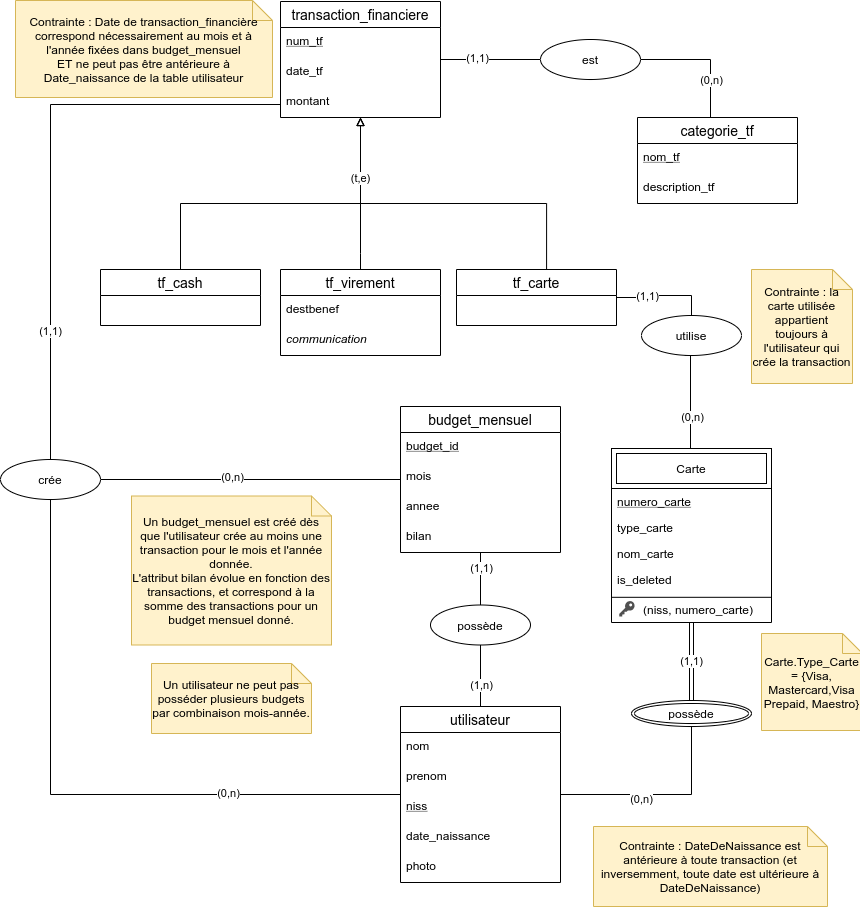
\includegraphics[scale=0.53]{ea_reg.png}}
\caption{\footnotesize{Schéma conceptuel entité-association de la base de données exploitée par Budget Squirrel}}
\end{figure}

\newpage 

\section{Schéma logique relationnel}

Vous trouverez ci-dessous notre traduction du schéma entité association présenté à la section précédente, ainsi que les contraintes qui lui sont liées, et quelques explications concernant nos choix de traduction.
Le schéma ci-dessous a été utilisé pour passer de notre schéma entité association au script SQL de création de base de données.

\begin{Verbatim}[commandchars=+\[\]]
utilisateur(nom, prenom, +underline[niss], date_naissance, photo)
	utilisateur.photo = {froggy.png, gollum.jpg, politecat.jpg, raccoon.jpg}

carte(nom_carte, +underline[numero_carte], type_carte, +underline[niss_util], is_deleted)
	carte.niss_util référence utilisateur.niss
	carte.type_Carte = {Visa, Mastercard,Visa Prepaid, Maestro}

budget_mensuel(+underline[budget_id], mois, annee, bilan, niss_util) 
	budget_mensuel.niss_util référence utilisateur.niss

transaction_financiere(+underline[num_tf], date_tf, montant, budget_id, niss_util, cat_tf)
	transaction_financiere.budget_id référence budget_mensuel.budget_id
	transaction_financiere.cat_tf référence categorie_tf.nom_tf
	transaction_fianciere.niss_util référence utilisateur.niss

tf_cash(+underline[num_tf])
	tf_cash.num_tf référence transaction_financiere.num_tf

tf_virement(+underline[num_tf], destbenef, +it[communication])
	tf_virement.num_tf référence transaction_financiere.num_tf

tf_carte(+underline[num_tf], +underline[numero_carte])
	tf_carte.num_tf référence transaction_financiere.num_tf	
	numero_carte référence carte.numero_carte

categorie_tf(+underline[nom_tf], description_tf)
\end{Verbatim}

Voici les contraintes que nous avons définies dans cette traduction, afin qu'elle corresponde à notre schéma entité-association :

\begin{itemize}
\item \verb\utilisateur.niss\ ne peut contenir que 11 caractères, spécifiquement 11 chiffres, pas plus, ni moins;
\item La valeur par défaut de \verb\carte.is_deleted\ est 0 (zéro);
\item La valeur de \verb\carte.numero_carte\ contient uniquement des chiffres, et ne peut contenir que 16 ou 17 chiffres;
\item \verb\budget_mensuel.budget_id\ correspond a une combinaison unique de \verb\niss_util\, \verb\mois\ et \verb\annee\, ainsi, il est impossible pour un même utilisateur de posséder plusieurs budgets pour le même mois et la même année;
\item \verb\budget_mensuel.bilan\ correspond à la somme de toutes les transactions pour un utilisateur, un mois et une année données;
\item \verb\transaction_financiere.date_tf\ (et par extension,  \verb\budget_mensuel.mois\ et \verb\budget_mensuel.annee\) sont nécessairement ultérieures à \verb\utilisateur.date_naissance\;
\item \verb\transaction_financiere.budget_id\ ne peut référencer qu'un \verb\budget_id\ dont le mois et l'année correspondent à \verb\transaction_financiere.date_tf\;
\item Dans la table \verb\tf_carte\, \verb\transaction_financiere.num_tf\ et \verb\carte.numero_carte\ référencent obligatoirement le même \verb\niss_util\ : un utilisateur ne peut qu'utiliser les cartes qui lui sont liées pour les transactions qui lui sont liées;
\item \verb\transaction_financiere.num_tf\ doit se retrouver une et une seule fois soit dans la table \verb\tf_carte\, soit dans la table \verb\tf_virement\, soit dans la table \verb\tf_cash\; 
\end{itemize}

L'héritage entre la table \verb\transaction_financiere\ et les tables \verb\tf_cash\, \verb\tf_virement\, et \verb\tf_carte\ a été traduit par une matérialisation, que nous représentons graphiquement à la figure \ref{materialisation}, en page \pageref{materialisation}.
Nous avons choisi d'utiliser la matérialisation afin de conserver la super-entité, les sous-entités, ainsi que la relation sémantique qu'elles entretiennent.
La relation est considérée comme totale et exclusive : une transaction financière est au moins une transaction en liquide, par virement ou payée par carte, mais ne peut pas être de plus d'un type à la fois.
Cela a donc nécessité l'ajout d'une contrainte spécifique.

L'association un à plusieurs entre \verb\utilisateur\ et \verb\budget_mensuel\ a été traduite en plaçant la référence du côté "un" de l'association : ainsi, on retrouve \verb\utilisateur.niss\ dans \verb\budget_mensuel.niss_util\.
Il en est de même pour la table \verb\transaction_financiere\, à laquelle nous avons ajouté une référence à la fois au \verb\budget_mensuel.budget_id\, et à \verb\utilisateur.niss\.
Toujours en suivant la même logique, l'entité faible \verb\carte\ contient son attribut d'association identifiante, lié au NISS de l'utilisateur, et la clé de la table est formée de la combinaison NISS - numéro de carte; la table \verb\transaction_financiere\ contient l'attribut qui référence \verb\categorie_tf.nom_tf\; et \verb\tf_carte\ contient les références à \verb\transaction_financiere.num_tf\ et à \verb\carte.numero_carte\. 

Nous n'avons pas dû traduire l'association ternaire entre \verb\transaction_financiere\, \verb\budget_mensuel\ et \verb\utilisateur\, tout simplement car elle n'est pas nécessaire : la table \verb\transaction_financiere\ contient déjà toutes les informations de l'association, à savoir l'association \verb\num_tf\ - \verb\budget_id\ - \verb\niss\. Une table séparée représentant le lien entre les trois tables aurait été nécessaire si, par exemple, des données étaient directement liée à l'association qui les lie, ou si l'on avait décidé de ne pas enregistrer le niss de l'utilisateur dans la table des transactions financières.

\begin{figure}[!ht]
\noindent
\makebox[\textwidth][c]{
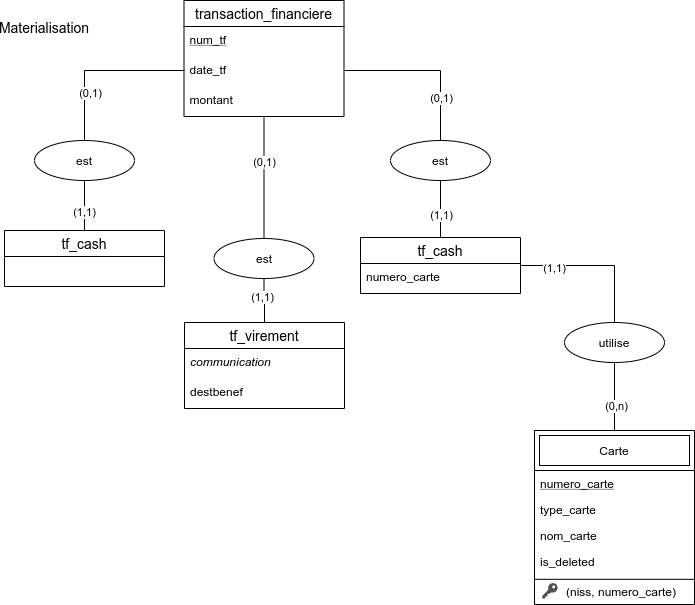
\includegraphics[scale=0.5]{mat_reg.png}}
\caption{\footnotesize{Matérialisation de l'héritage entre les transactions}}
\label{materialisation}
\end{figure}

\newpage

\section{Code SQL}

Dans cette section, nous présentons les différents éléments de SQL qui sont présents dans notre projet, ainsi que leur utilité respective.
Comme décrit dans notre introduction, vous trouverez en annexe deux fichiers SQL : \verb\initdb.sql\, et \verb\basicdata.sql\. Le premier contient le script de création des tables, la mise en place des déclencheurs, la création des vues, et enfin la définition des utilisateurs et de leurs privilèges respectifs. Le second peuple les différentes tables, en ajoutant : 3 utilisateurs, 2 ou 3 cartes par utilisateur, les catégories de transaction et leur description, et quelques transactions pour chaque utilisateurs.

Ainsi, une fois les deux scripts SQL exécutés, l'application peut être utilisée et des données d'exemple sont déjà disponibles.

\subsection{Description du code de création de la base de données}

Après une requête de suppression de la base de données \verb\budgetsquirrel\ si elle existe déjà, une nouvelle base de données du même nom est créée et appelée à être utilisée.
Les premières requêtes sont des \verb\CREATE TABLE\, et permettent de créer les tables qui sont nécessaires à l'utilisation de l'application. Elles correspondent à notre schéma logique relationnel. Ainsi, le script SQL crée les tables suivantes : \verb\utilisateur\, \verb\carte\, \verb\budget_mensuel\, \verb\categorie_tf\, \verb\transaction_financiere\, \verb\tf_cash\, \verb\tf_virement\, et \verb\tf_carte\.

Les contraintes prévues par le schéma logique relationnel pouvant être traduites directement dans la création des tables sont alors établies. Tous les attributs obligatoires sont déclarés comme non nuls et la longueur de \verb\utilisateur.niss\ est fixée à 11, la longueur de \verb\carte.numero_carte\ est fixée entre 16 et 17, grâce à des \verb\CHECK\ que nous décrivons plus loin (vu que ce ne sont pas des chiffres sur lesquels il faut faire des calculs, ces données sont enregistrées en \verb\VARCHAR\, de manière similaire à des numéros de téléphone).
Toutes les clés primaires et étrangères sont également déclarées dans cette partie du script.
Lorsque cela est nécessaire, nous ajoutons des contraintes \verb\UNIQUE\, toujours pour respecter notre schéma : c'est le cas pour la contrainte \verb\carte.uc_carte\, \verb\utilisateur.uk_utilisateur\, et \verb\uc_budget_mensuel\.

Dans la table \verb\budget_mensuel\ comme dans la table \verb\transaction_financiere\, nous utilisons la commande \verb\AUTO_INCREMENT\ afin d'établir que les clés primaires de ces tables, à savoir \verb\budget_mensuel.budget_id\ et \verb\transaction_financiere.num_tf\, sont des colonnes numériques qui sont incrémentées automatiquement à chaque nouvelle insertion.

Nous avons également ajouté quelques contraintes liées à notre application. Par exemple, nous donnons une valeur par défaut à l'url de la photo (\verb\utilisateur.photo\), et nous établissons que les seules valeurs acceptées par l'attribut \verb\utilisateur.photo\ sont celles correspondant aux photos de notre dossier d'images. De manière similaire, nous établissons que les seules valeurs acceptées pour \verb\carte.type_carte\ sont Visa, Mastercard, Visa Prepaid, et Maestro. De plus, une carte créée est par défaut considérée comme non supprimée, ainsi, \verb\carte.is_deleted\ a une valeur par défaut de 0. 

Puisque l'utilisateur peut supprimer ses transactions, nous avons ajouté des \verb\ON DELETE CASCADE\ aux \verb\num_tf\ référencés dans les tables \verb\tf_cash\, \verb\tf_virement\, et \verb\tf_carte\, afin que la transaction soit supprimée des tables qui contiennent des informations sur son type.
Un administrateur pourrait éventuellement vouloir supprimer totalement un utilisateur de la base de données, lui et toutes ses cartes, transactions, ou encore changer certaines informations liées à ce dernier, et que cela se répercute sur le reste de la base de données.
Afin de gérer ces deux situations, nous avons ajouté des  \verb\ON DELETE CASCADE\ et des \verb\ON UPDATE CASCADE\ à chaque référence du NISS de l'utilisateur en tant que clé étrangère.

Après la création des tables que nous venons de présenter, \verb\initdb.sql\ peut être divisé en 3 grandes parties : la création des triggers/déclencheurs, la création des vues, et la gestion des privilèges.
Toutes ces parties sont décrites dans les points suivants.

\subsection{Éléments de SQL avancé}

Vous trouverez dans les points suivants la description de divers éléments de SQL avancé auxquels nous avons fait appel dans le cadre de notre projet.

\subsubsection{Contraintes garanties par des check}

Comme décrit précédemment, nous faisons appel à des \verb\CHECK\ afin de vérifier la validité de certaines valeurs d'attributs dans notre base de données.
Il y a en tout 5 checks : \verb\chk_niss\, qui vérifie que le NISS enregistré fait bien la bonne longueur (exactement 11 chiffres) \verb\chk_photo\, qui vérifie que la valeur de la photo est bien une de celles que nous avons définies, \verb\chk_numero_carte_low\ et \verb\chk_numero_carte_high\, qui vérifient que le numéro de carte entré correspond bien à la longueur demandée (entre 16 et 17 chiffres), et enfin, \verb\chk_type_carte\, qui vérifie que \verb\type_carte\ correspond bien aux différents types de cartes définis précédemment. 

\subsubsection{Requêtes de consultation}

Nous faisons appel à de nombreuses requêtes de consultation plus ou moins complexes dans le cadre de notre système : nous faisons appel à des \verb\SELECT\ tout au long de l'application pour récupérer différentes informations (noms d'utilisateurs, cartes, historique...), mais également dans les vues que nous décrirons plus loin, afin de sélectionner les informations nécessaire à la création de ces dernières. 

\subsubsection{Requêtes de mise à jour}

Des requêtes \verb\UPDATE\ sont également utilisées : dans l'application, nous faisons appel à ces dernières pour mettre à jour le statut des cartes et changer la photo de profil de l'utilisateur.
Du côté du système de gestion de base de données, les \verb\UPDATE\ sur d'autres données sont rendus possible grâce à l'ajout de \verb\ON UPDATE CASCADE\ sur différentes données. 
Ainsi, il est possible pour l'administrateur de supprimer des utilisateurs s'il le souhaite, ou encore d'en modifier des informations comme le NISS, et que ces valeurs se répercutent sur le reste de la base de données.

\subsubsection{Vues utilisées}

La base des données contient quatre vues qui sont utilisées dans la construction d'historiques et de statistiques dans l'application : 

\begin{enumerate}
\item historique\textunderscore v, qui liste chronologiquement les informations liés aux transactions effectuées par un utilisateur,
\item stat\textunderscore depenses\textunderscore revenus\textunderscore mois, qui liste chronologiquement les dépenses et les revenus enregistrés par l'utilisateur, en faisant également le bilan des dépenses, le bilan des revenus, et le bilan total,
\item stat\textunderscore cat, qui liste la répartition totale des dépenses et des revenus par catégorie et par utilisateur, 
\item et stat\textunderscore types, qui liste la répartition du budget global par type de transaction employé dans le payement, ainsi que par nombre d'emplois de chaque type de transaction, pour un bilan global des dépenses et revenus.
\end{enumerate}

Ces vues sont utiles à la gestion et à l’agrégation des données, et permettent notamment d'offrir à l'utilisateur de l'application différents graphiques et informations agrégées sur son budget.
Leur création est appelée juste après la création des triggers dans \verb\initdb.sql\.

Ci-dessous, vous trouverez une description détaillée de leur fonctionnement.

\paragraph{Historique}\mbox{}\\
La vue \verb\historique_v\ est notre vue principale, sur base de laquelle les autres vues sont générées.
Elle permet de rassembler toutes les informations pour une transaction donnée dans une seule table.
Son résultat permet ainsi de consulter, pour chaque transaction : son identifiant, sa date, son montant, le NISS de l'utilisateur à laquelle elle est liée, l'identifiant de budget auquel elle est liée, sa catégorie, et éventuellement: le numéro et le nom de la carte utilisée, le destinataire/bénéficiaire et la communication.
Le type est défini en utilisant un \verb\CASE\ : si \verb\num_tf\ est dans la table \verb\transaction_financiere\ et dans la table \verb\tf_virement\, la colonne \verb\typetf\ est remplie pour ce \verb\num_tf\ par \og virement\fg, et ainsi de suite pour les autres types de transaction.
Ensuite, des \verb\LEFT JOIN\ permettent de combiner les informations liées aux tables \verb\transaction_financiere\, \verb\tf_carte\, \verb\tf_cash\ et \verb\tf_virement\ sans perdre d'informations.
Finalement, cette vue permet de compléter la table \verb\transaction_financiere\ des données supplémentaires liées aux sous-tables de type, et ce pour chaque transaction effectuée.

\paragraph{Statistiques mensuelles}\mbox{}\\
La vue \verb\stat_depenses_revenus_mois\ a pour objectif de donner les informations suivantes par mois et par utilisateur : l'identifiant de budget, le mois, l'année, le bilan, le nombre de transactions effectuées, le total des dépenses et des revenus.
Cette vue est générée à partir de 3 \verb\SELECT\ basés sur la vue \verb\historique_v\ : un qui reprend les transactions dans leur ensemble, un autre qui ne reprend que les dépenses, et un autre qui ne reprend que les revenus.

\paragraph{Statistiques par catégorie}\mbox{}\\
L'objectif de la vue est d'obtenir des informations sur la répartition des transactions des utilisateurs par catégories : combien de fois elles ont été appelées pour les dépenses, pour les revenus, ainsi que la somme des dépenses et revenus les concernant.
Pour ce faire, un \verb\SELECT\ est fait entre la table des catégories et un \verb\SELECT\ de \verb\historique_v\.
Ce dernier récupère \verb\historique_v.cat_tf\ et \verb\historique_v.niss_util\, compte le nombre d'utilisations par catégories, fait la somme des montants négatifs, celle des montants positifs, et groupe le tout par catégorie et par utilisateur.

\paragraph{Statistiques par type de transaction}\mbox{}\\
Afin d'obtenir une vue répartissant les transactions en fonction de leur type, nous mettons en place une vue agrégeant les information de la vue \verb\historique_v\.
La vue est assez simple, et fait un \verb\SELECT\ et un \verb\COUNT\ de \verb\historique_v.type_tf\, ainsi qu'un \verb\SELECT\ de \verb\historique_v.niss_util\.
Ensuite, elle calcule deux sommes, en fonction de la nature positive ou négative de chaque montant : le total des dépenses pour un type donné, et le total des revenus pour un type donné.

\subsubsection{Déclencheurs}

Afin de conserver toutes les contraintes définies dans notre schéma, nous avons défini 7 déclencheurs : \verb\trg_before_ajout_tf\, \verb\trg_after_ajout_tf\, \verb\trg_after_suppr_tf\, \verb\trg_before_ajout_tf_carte_niss\, \verb\trg_before_ajout_tf_carte\, \verb\trg_before_ajout_tf_cash\, et \verb\trg_before_ajout_tf_virement\. La création de ces déclencheurs suit directement la création des tables, et permet, entre autres, d'établir les contraintes les plus complexes (qui incluent les informations de plusieurs tables). Nous expliquons le fonctionnement de chacun des ces déclencheurs dans les points suivants.

\paragraph{Vérifier les informations avant l'ajout d'une transaction financière}\mbox{}\\
Le déclencheur \verb\trg_before_ajout_tf\, qui se fait avant chaque insertion sur la table \verb\transaction_financiere\, permet de vérifier plusieurs informations.
Tout d'abord, une vérification sur la date est faite : si la date de transaction est antérieure à la date de naissance de l'utilisateur, un message d'erreur est renvoyé et la transaction ne s'enregistre pas.
Ensuite, l'objectif est de trouver le \verb\budget_id\ à lier à la transaction financière à créer.
Pour ce faire, nous vérifions d'abord, via un \verb\SELECT\, qu'il existe déjà un \verb\budget_mensuel\ correspondant à la combinaison de mois, d'année et de NISS.
Si ce n'est pas le cas (que le résultat \verb\COUNT(*)\ = 0), le \verb\budget_mensuel\ correspondant est créé.
Ensuite, dans tous les cas, le \verb\budget_id\ du \verb\budget_mensuel\ correspondant est sélectionné, et défini comme à écrire dans l'insertion de la nouvelle \verb\transaction_financiere\.
Ce trigger permet donc de conserver nos contraintes de dates, autant par rapport à la date de naissance de l'utilisateur, qu'au fait que la date d'une transaction correspond nécessairement au mois et à l'année d'un budget mensuel donné (ainsi qu'au NISS de l'utilisateur qui l'a créée).

\paragraph{Écrire (et réécrire) le bilan du budget mensuel en cas d'insertion ou de suppression dans la table des transactions financières}\mbox{}\\
Deux déclencheurs sont utilisés pour que \verb\budget_mensuel.bilan\ corresponde toujours à la bonne somme de transactions : \verb\trg_after_ajout_tf\ et \verb\trg_after_suppr_tf\.
Dans les deux cas, après une insertion ou une suppression de la table \verb\transaction_financiere\, le résultat \verb\bilan_total_mois\ de la vue \verb\stat_depenses_revenus_mois\ correspondant au \verb\budget_id\ et au \verb\niss_utilisateur\ de l'insertion ou de la suppression est sélectionné, et permet de faire une modification de \verb\budget_mensuel.bilan\.

\paragraph{Vérifier que la carte utilisée lors de la transaction appartient bien à l'utilisateur}\mbox{}\\
Lors de l'ajout d'une transaction dans la table \verb\tf_carte\, il est important, afin de respecter une des contraintes que nous avions définies, de vérifier que la carte qui est utilisée appartient bien à l'utilisateur qui a fait la transaction.
Le déclencheur \verb\trg_before_ajout_tf_carte_niss\, avant l'insertion dans la table enregistrant les transactions par carte, va donc récupérer le NISS présent dans la table des transactions financières créées qui correspond au bon numéro de transaction, et le NISS correspondant à la carte utilisée.
Si les deux NISS récupérés diffèrent, un message d'erreur s'affiche, et l'enregistrement ne se fait pas dans la table \verb\tf_carte\.

\paragraph{Conserver la contrainte d'héritage total et exclusif}\mbox{}\\
Afin d'assurer que les transactions financières ne sont pas écrites plusieurs fois, mais bien une seule, dans une des trois tables qui définissent leur type (\verb\tf_carte\, \verb\tf_virement\ et \verb\tf_cash\), nous utilisons trois triggers :  \verb\trg_before_ajout_tf_carte\, \verb\trg_before_ajout_tf_cash\, et \verb\trg_before_ajout_tf_virement\.
Chacun de ces déclencheurs fait la même vérification avant ajout. Grâce à des \verb\SELECT\ dans les deux autres tables, s'il existe déjà une ligne qui correspond au numéro de transaction, l'ajout dans la table de type ne se fait pas, et un message apparaît.

\subsubsection{Droits d'accès}

Enfin, le script \verb\initdb.sql\ définit également deux utilisateurs principaux, ainsi que leurs privilèges.
Nous y définissons deux utilisateurs : \verb\utilisateur_app\, qui est celui qui est appelé tout au long de l'application, et \verb\utilisateur_admin_db\, qui, comme son nom l'indique, est l'utilisateur-administrateur.
Alors que ce dernier a un accès illimité à la base de données (défini grâce à \verb\GRANT ALL PRIVILEGES\), \verb\utilisateur_app\ ne peut faire que les actions définies par le script.

Les actions définies sont les suivantes, et correspondent aux actions rendues possibles par l'utilisation de l'application : 
\begin{itemize}
\item L'insertion, la modification et la sélection de lignes pour la table \verb\utilisateur\, ce qui lui permet de s'inscrire, de modifier ses informations, et de pouvoir avoir accès à la liste des utilisateurs (cf. écran de connexion) ainsi qu'à ses informations;
\item le droit de sélection et d'insertion sur la table \verb\transaction_financiere\, ce qui lui permet de visualiser et d'insérer de nouvelles transactions financières;
\item le droit à la sélection et à l'insertion dans la table \verb\budget_mensuel\ (le droit à la sélection n'est pas réellement nécessaire, vu que le trigger \verb\trg_before_ajout_tf\ automatise l'écriture des budgets mensuels);
\item le droit à la sélection, la modification et l'insertion pour la table carte, afin de pouvoir utiliser, supprimer/désactiver, et créer ses cartes;
\item le droit de sélection sur la table \verb\categorie_tf\, afin de définir la catégorie d'une transaction, et pouvoir consulter la description d'une catégorie sélectionnée dans son tableau statistique;
\item   le droit de sélection des différentes vues que nous avons créées (\verb\stat_depenses_revenus_mois\, \verb\historique_v\, \verb\stat_cat\ et \verb\stat_types\), afin d'avoir accès aux parties de l'application qui rassemblent des statistiques sur ses transactions;
\end{itemize}


\section{Description de l'application Web}

L'application web que nous avons développée a pour objectif de permettre aux utilisateurs de s'inscrire, d'enregistrer leurs transactions, de consulter leur historique par mois, ainsi que des statistiques diverses sur la répartition de leurs dépenses, de leur revenus, et un bilan total de leur budget. 
L'accès à la base de données est restreint : ce n'est pas un accès root, mais bien un accès spécifiquement défini pour les utilisateurs de l'application. Nous en avions fait la description détaillée à la section précédente.

L'application contient 9 pages : \verb\index.html\, \verb\inscription.php\, \verb\connexion.php\, \verb\homepage.php\, \verb\profil.php\, \verb\historique.php\, \verb\enregistrement.php\, \verb\stat.php\, et \verb\logout.php\. Ci-dessous, nous en décrivons leur articulation.

À l'ouverture de l'application (\verb\localhost/budgetsquirrel/index.html\ ou simplement \verb\localhost/budgetsquirrel/\), l'utilisateur a deux possibilités : se connecter, ou s'inscrire.

\begin{figure}[!ht]
\noindent
\makebox[\textwidth][c]{

\includegraphics[scale=0.25]{index.png}}
\caption{\footnotesize{Landing page - Budget Squirrel}}
\end{figure}

S'il choisit de s'inscrire, il est redirigé vers un formulaire d'inscription, \verb\inscription.php\, où il doit rentrer son nom, son prénom, son NISS, et choisir une photo de profil.
Si toutes les informations ne sont pas complétées, l'utilisateur est notifié du fait qu'il doit rentrer toutes les informations pour pouvoir s'inscrire.

\begin{figure}[!ht]
\noindent
\makebox[\textwidth][c]{
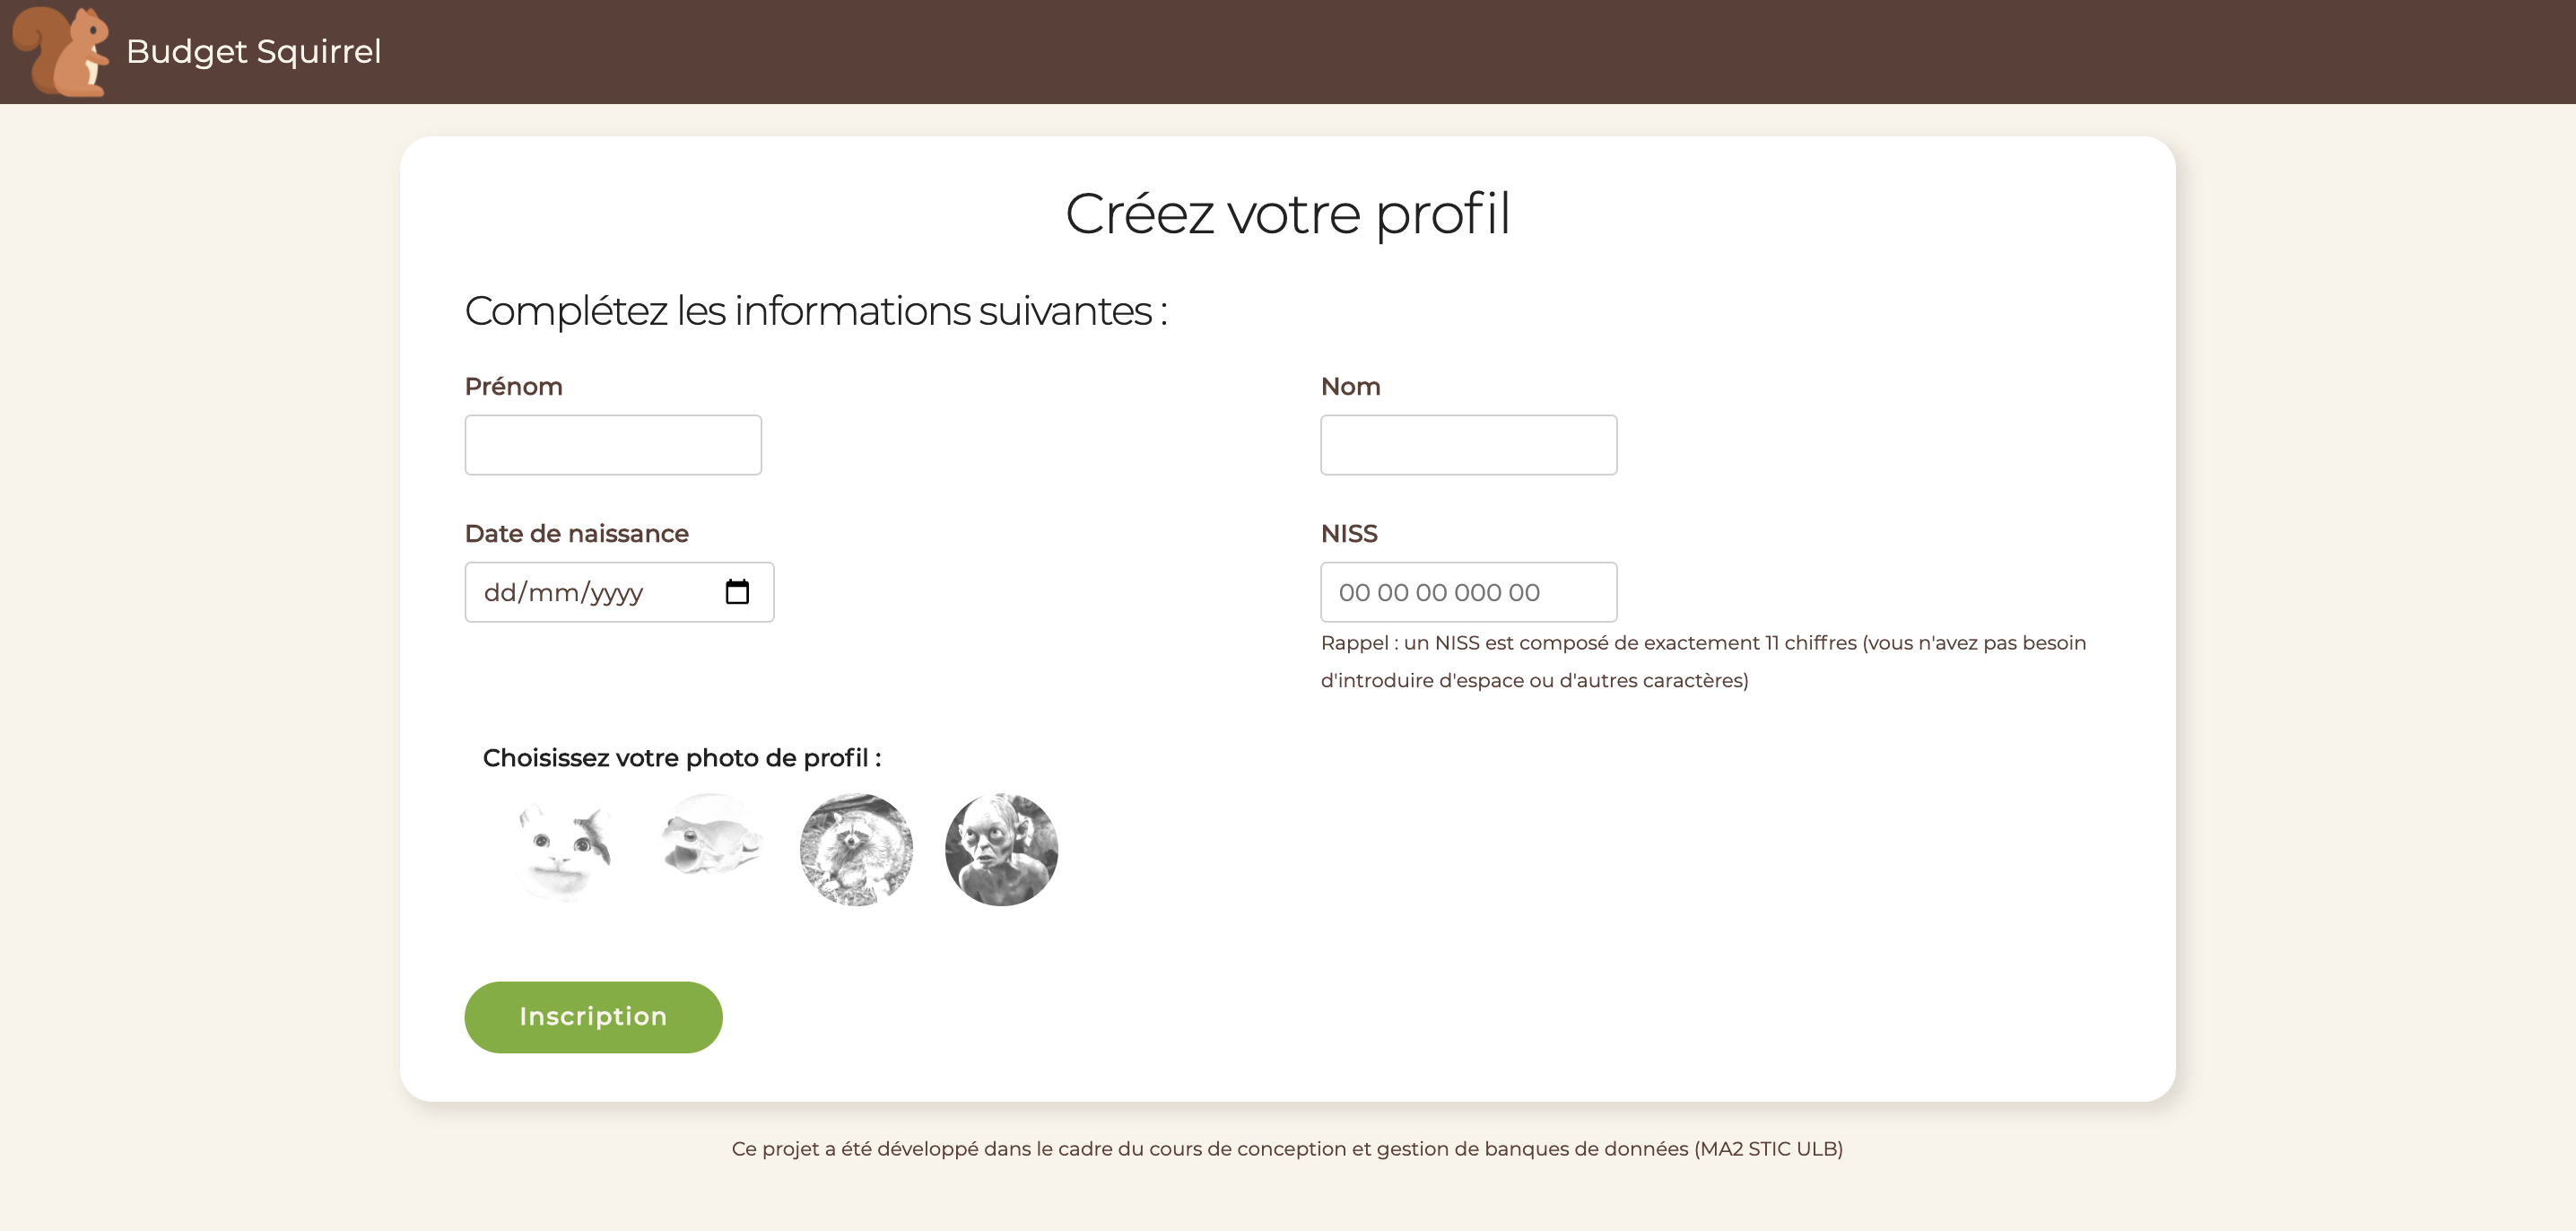
\includegraphics[scale=0.25]{inscription.png}}
\caption{\footnotesize{Écran d'inscription - Budget Squirrel}}
\end{figure}

Si un utilisateur est déjà inscrit sous le NISS entré, il en est notifié (et a la possibilité de se rediriger vers la page de connexion).
Si le NISS n'est pas encore utilisé par un utilisateur, l'enregistrement se fait, l'utilisateur est notifié du succès de ce dernier, et il peut se rediriger vers la page de connexion.
La vérification de la présence d'un utilisateur utilisant déjà le NISS se fait à deux niveaux : au niveau de la base de données en elle-même, comme nous l'avons vu au dessus, grâce à la contrainte de clé primaire, et également en PHP, en faisant une sélection de la table utilisateur (si la sélection par rapport au NISS entré renvoie un résultat différent de zéro, l'utilisateur est notifié de l'impossibilité de créer un compte avec ce NISS).

La page de connexion \verb\connexion.php\, par souci de simplification, est une simple sélection de profil : l'utilisateur a accès à la liste des utilisateurs, sélectionne son profil (nom et prénom) dans la liste, et se connecte.
Ensuite, le NISS de l'utilisateur est récupéré par une méthode POST, enregistré par la méthode \verb\SESSION\ et appelé grâce à \verb\session_start();\ à chaque page de l'application où il est enregistré comme connecté.

\begin{figure}[!ht]
\noindent
\makebox[\textwidth][c]{
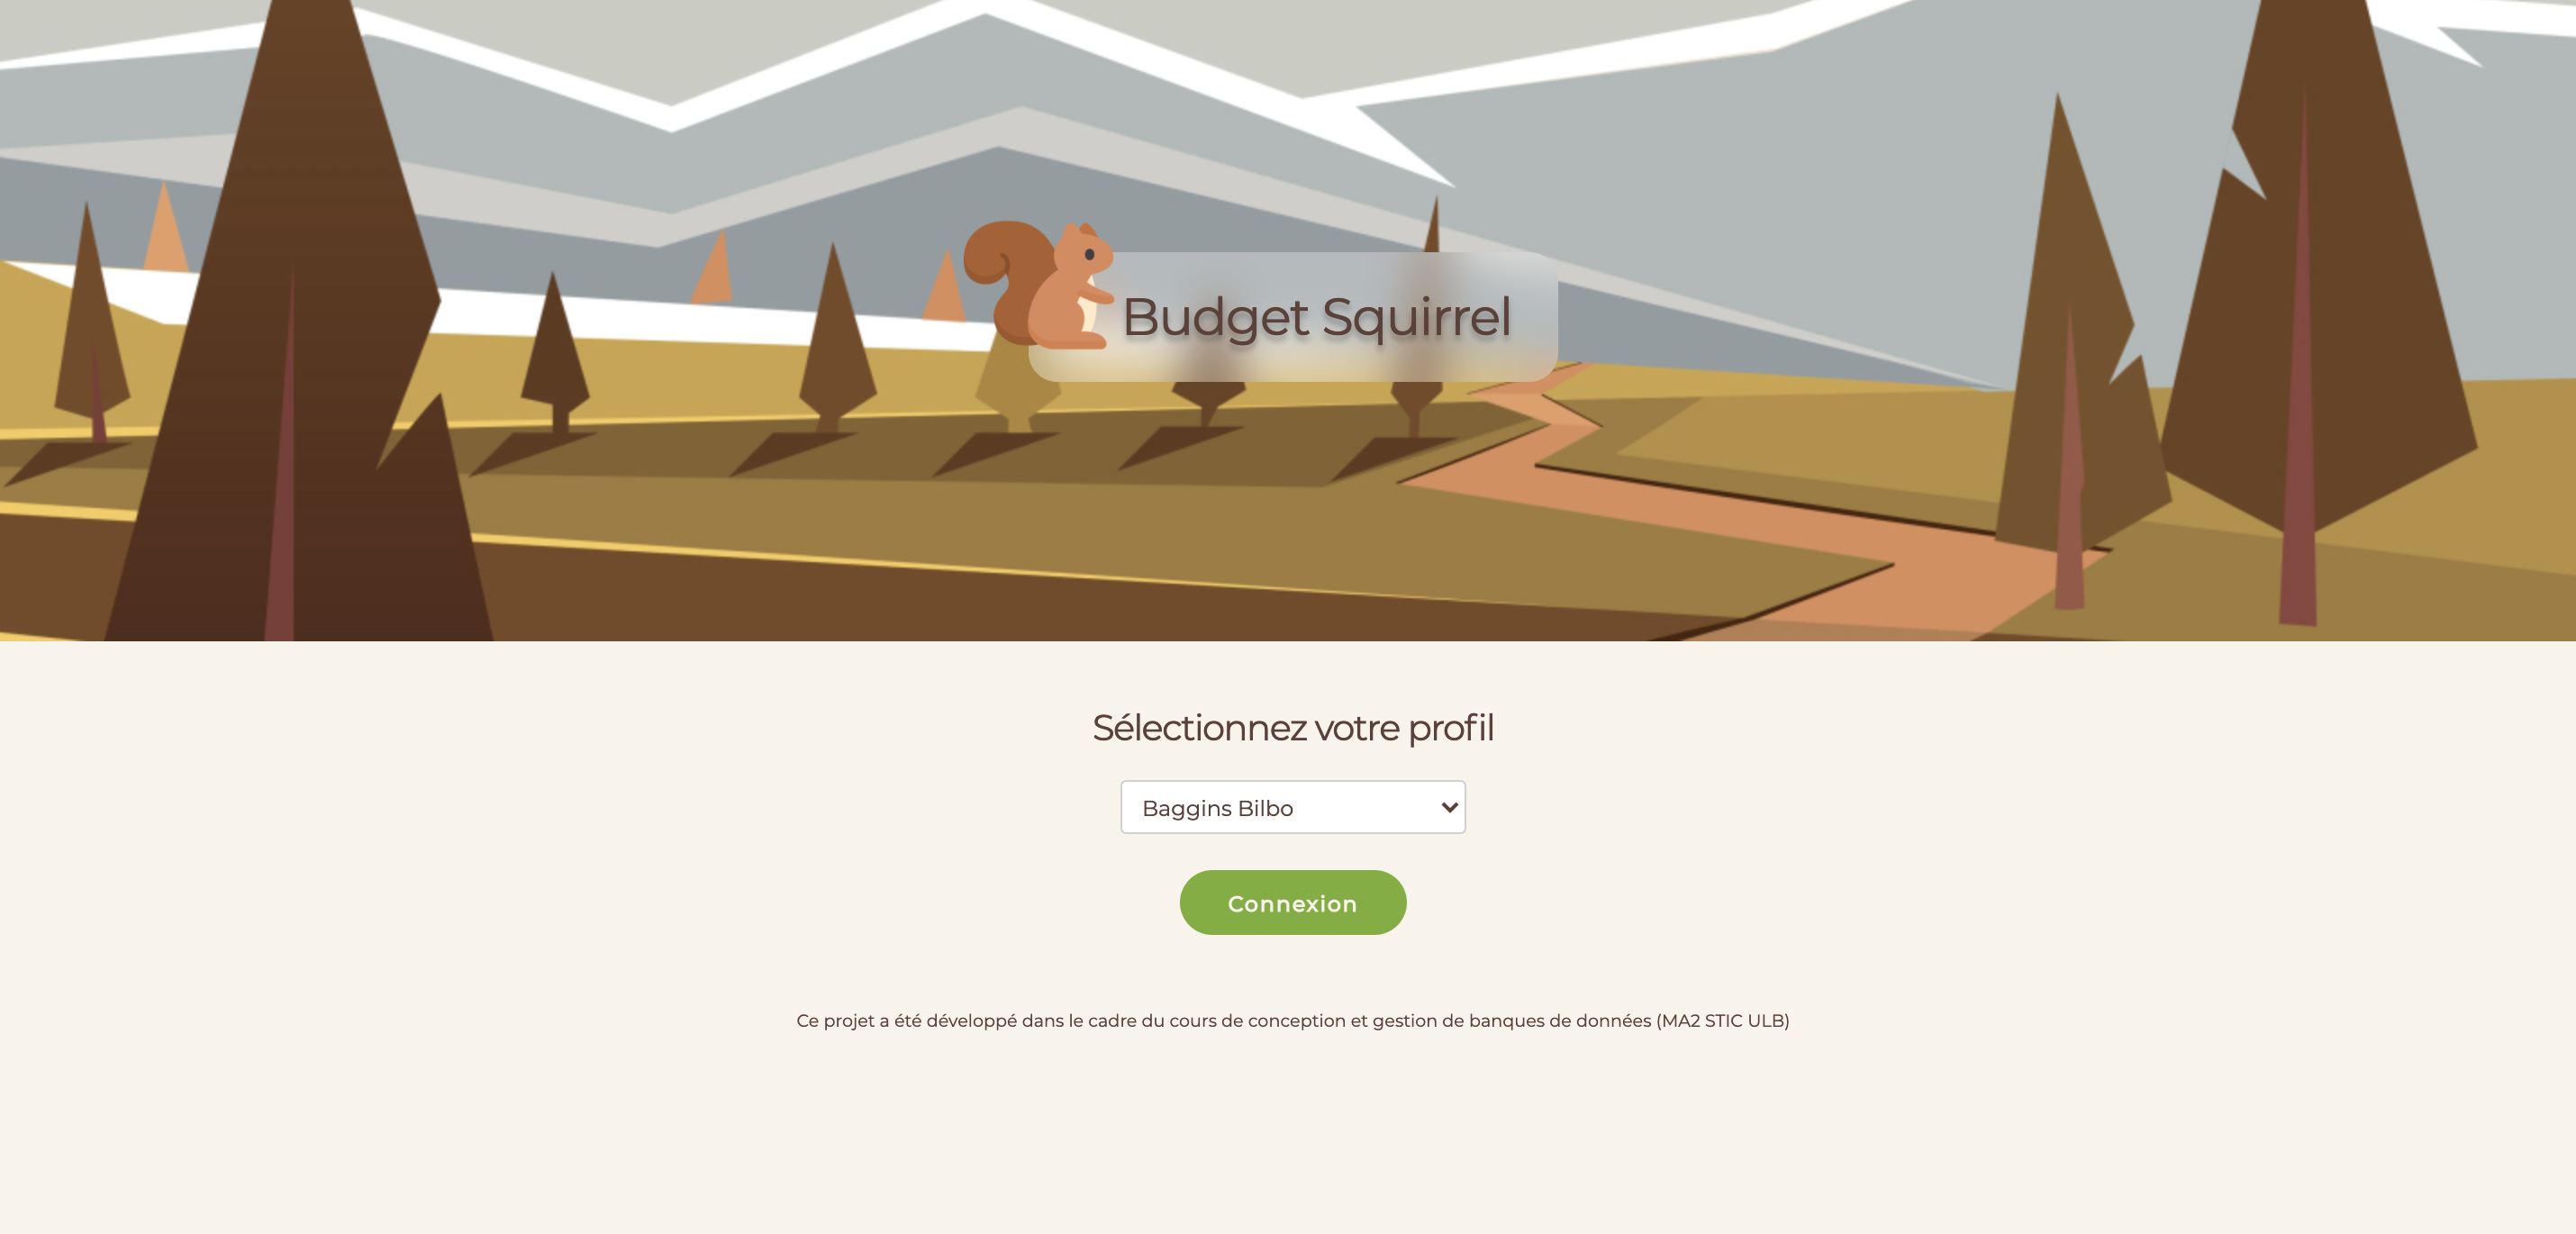
\includegraphics[scale=0.3]{connexion.png}}
\caption{\footnotesize{Écran de connexion - Budget Squirrel}}
\end{figure}

Une fois qu'il a sélectionné son profil et choisi de se connecter, l'utilisateur est redirigé vers une page d'accueil, \verb\homepage.php\.
La page d'accueil présente brièvement les différentes pages de l'application.
Depuis la barre de navigation, visible sur toutes les pages (sauf celles ou l'utilisateur n'est pas considéré comme connecté), l'utilisateur a accès : à la page d'accueil, à l'historique, à la page d'enregistrement, à la page de statistiques, et à sa page personnelle de profil.
Il peut ainsi naviguer librement entre les différentes pages de l'application.

\begin{figure}[!ht]
\noindent
\makebox[\textwidth][c]{
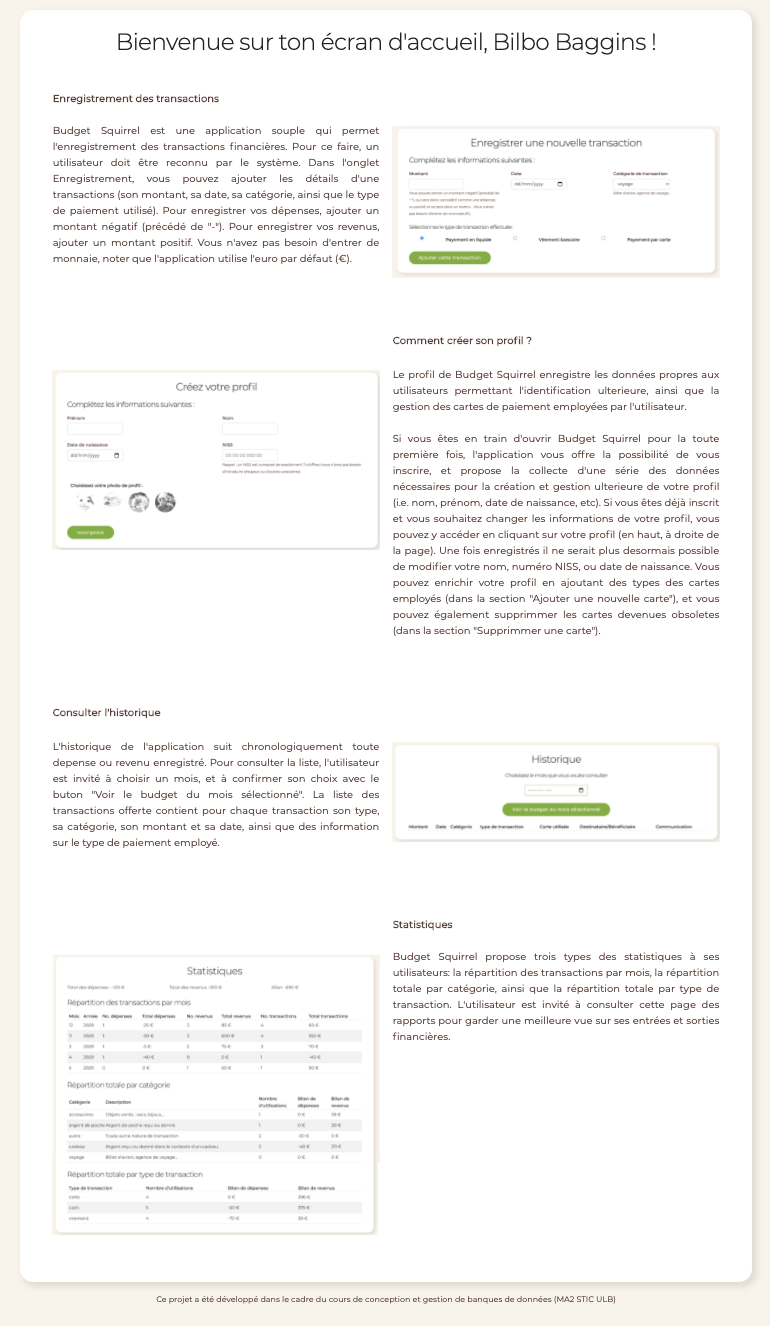
\includegraphics[scale=0.8]{homepage.png}}
\caption{\footnotesize{Page d'accueil - Budget Squirrel}}
\end{figure}

\newpage
La page personnelle de profil, \verb\profil.php\, permet à l'utilisateur de visualiser ses informations : nom, prénom, NISS, date de naissance.
Il peut également y ajouter et y supprimer ses cartes\footnote{Cette suppression est, comme nous l'avions expliqué, une suppression logique du côté de la base de données : les cartes possèdent une colonne is\_deleted\, par défaut la valeur de la colonne est à 0, et si l'utilisateur \og supprime\fg sa carte, la valeur passe à 1, et la carte est considérée comme virtuellement supprimée}.
Les listes de ses cartes disponibles et de ses anciennes cartes sont également visibles depuis la page de profil.
Il peut également y actualiser sa photo de profil.

\begin{figure}[!ht]
\noindent
\makebox[\textwidth][c]{
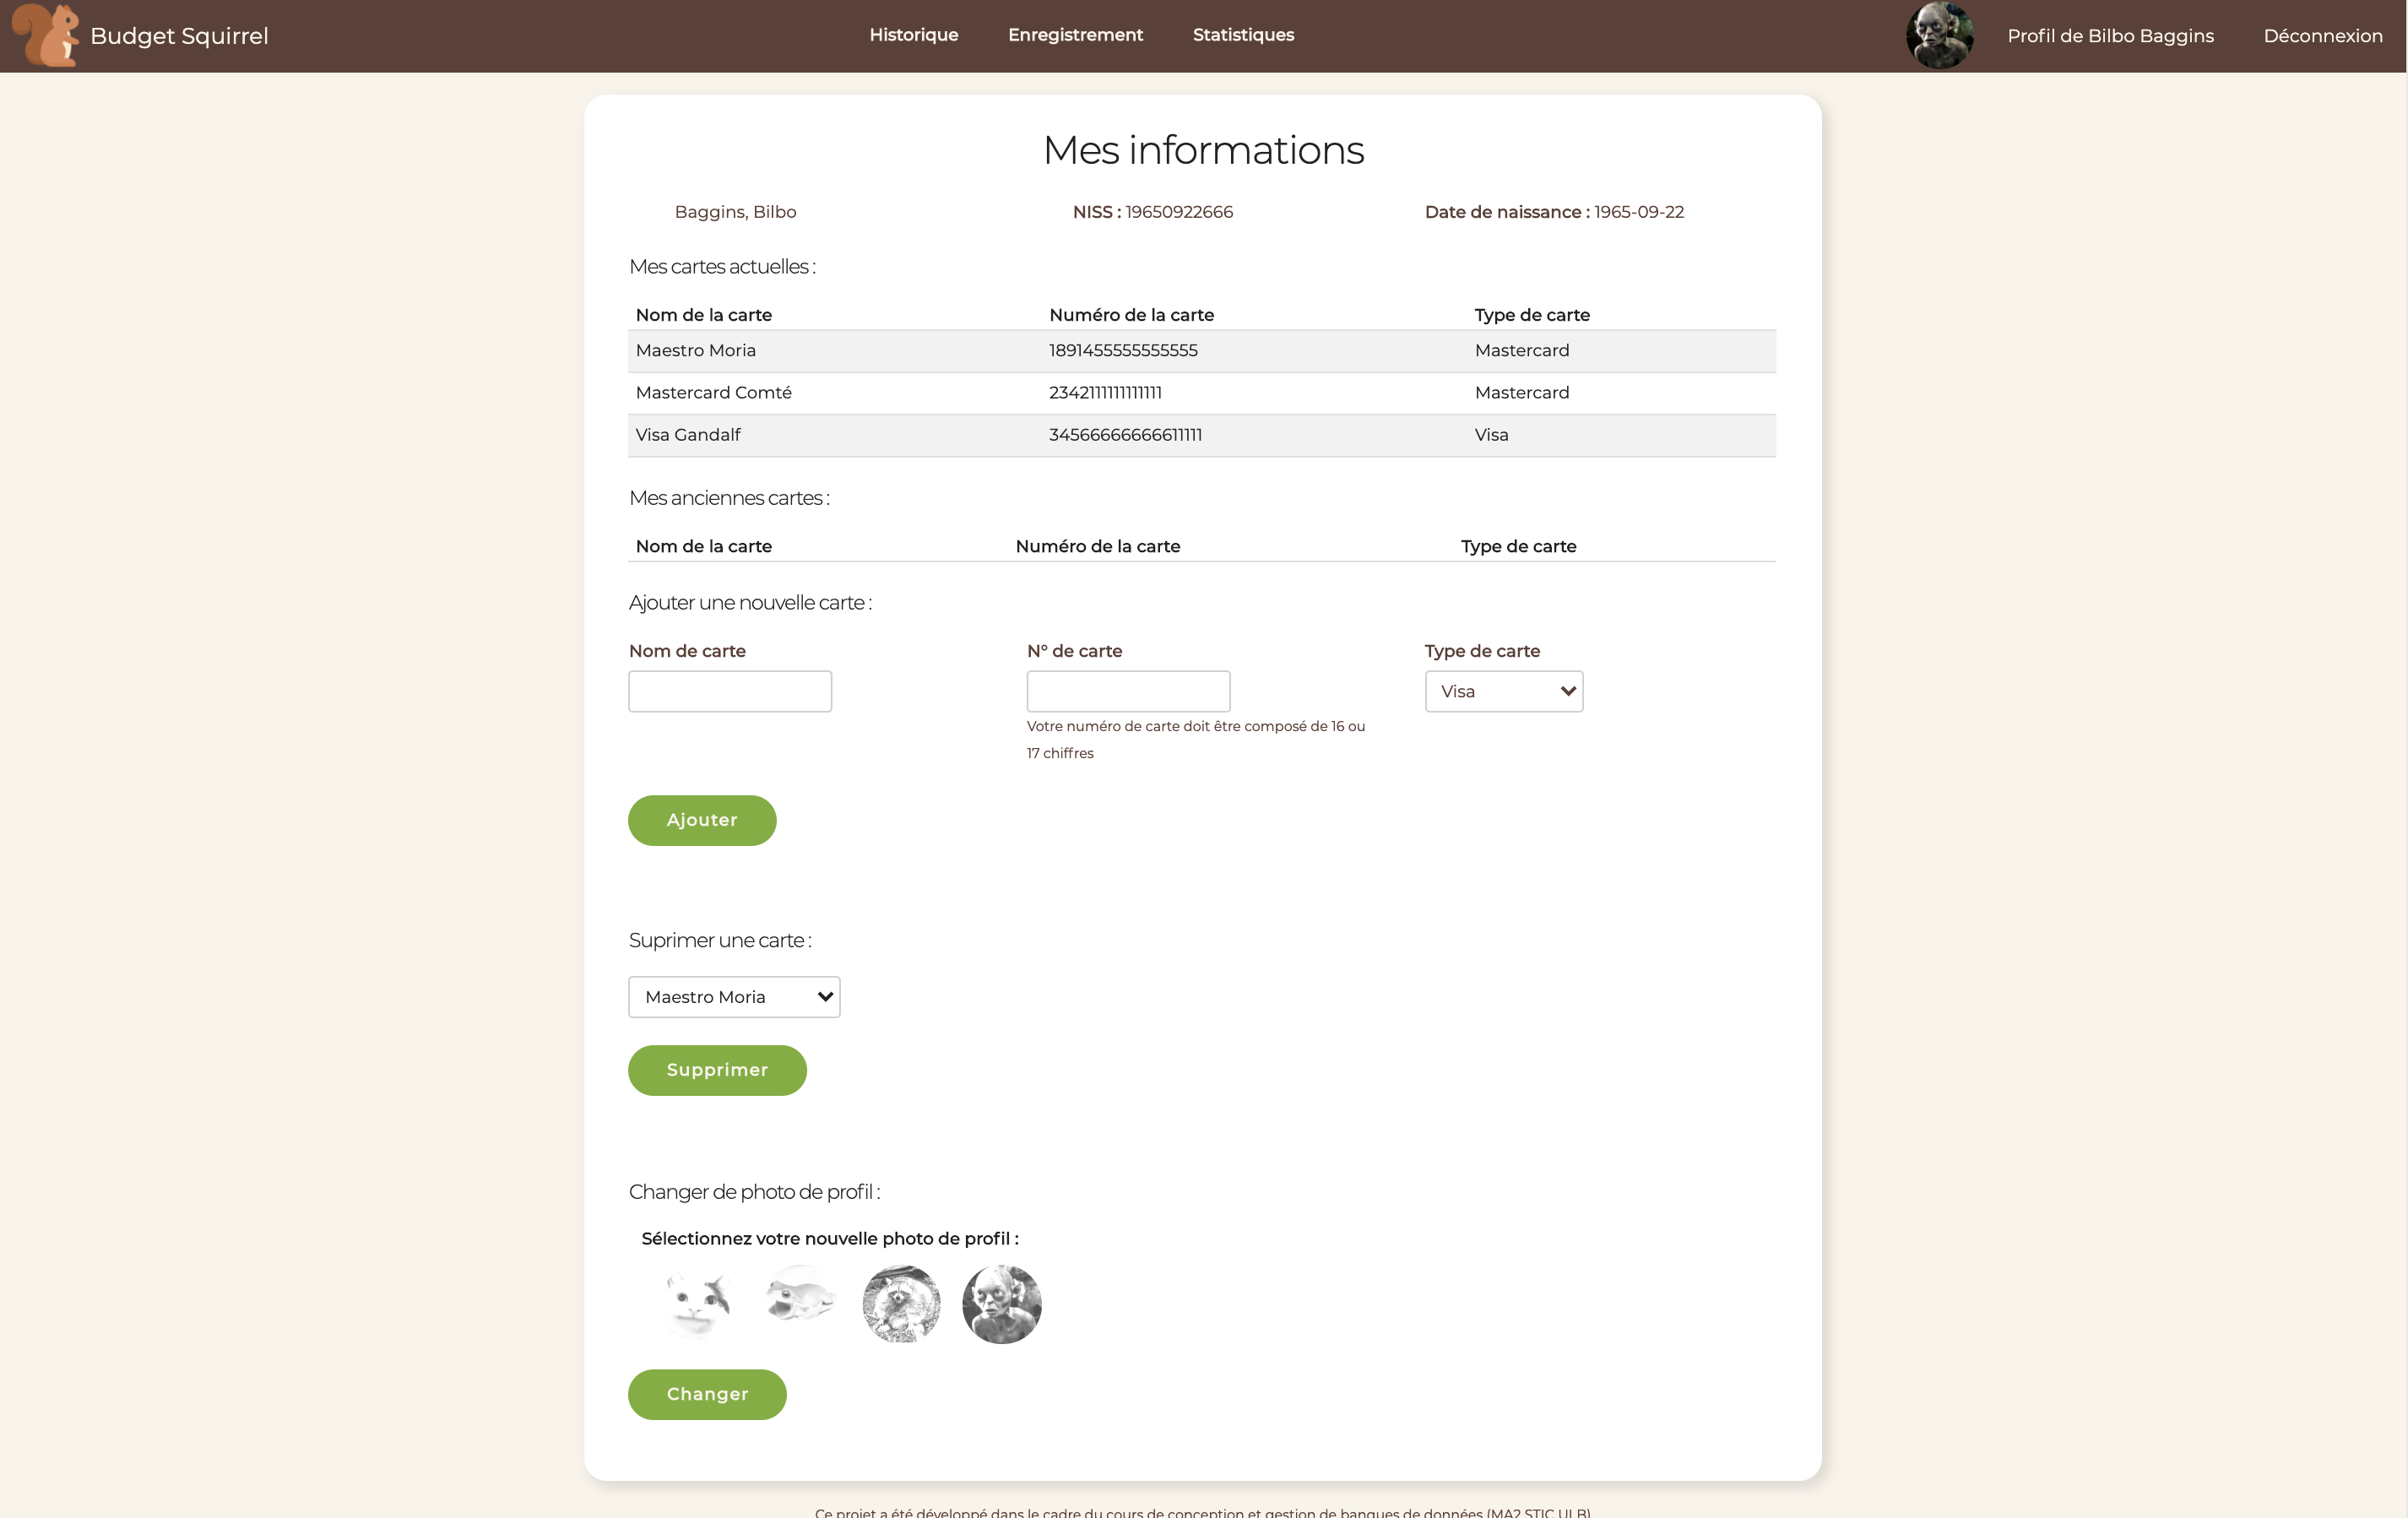
\includegraphics[scale=0.25]{profil.png}}
\caption{\footnotesize{Page personnelle - Budget Squirrel}}
\end{figure}

La page d'enregistrement, \verb\enregistrement.php\, permet d'enregistrer des transactions.
L'utilisateur est obligé d'entrer un montant, de sélectionner une date, une catégorie de transaction, et un type de transaction (à nouveau, la vérification se fait une fois en PHP, et une fois aussi du côté de la base de données).

En fonction du type de transaction effectuée, il doit également ajouter des informations supplémentaires, qui permettent de faire l'écriture dans la bonne table de type de transaction.
L'utilisateur sélectionne, via un radio button, le type de transaction effectuée : soit un payement en liquide, soit un virement bancaire, soit un payement par carte (JavaScript nous permet de cacher une partie du formulaire en fonction du radio button sélectionné).
Le payement en liquide ne demande aucune information supplémentaire, le virement bancaire demande d'introduire un destinataire ou un bénéficiaire, et éventuellement une communication, et un payement par carte nécessite de sélectionner la carte utilisée.
Cet aspect est géré uniquement en PHP, et demande donc de faire deux opérations consécutives si l'on veut rentrer le type de transaction sans passer par l'application Web : d'abord, un \verb\INSERT\ dans la table \verb\transaction_financiere\, puis un autre \verb\INSERT\ dans la table correspondant au bon type de transaction (c'est également ce que nous faisons dans \verb\basicdata.sql\).

\begin{figure}[!ht]
\noindent
\makebox[\textwidth][c]{
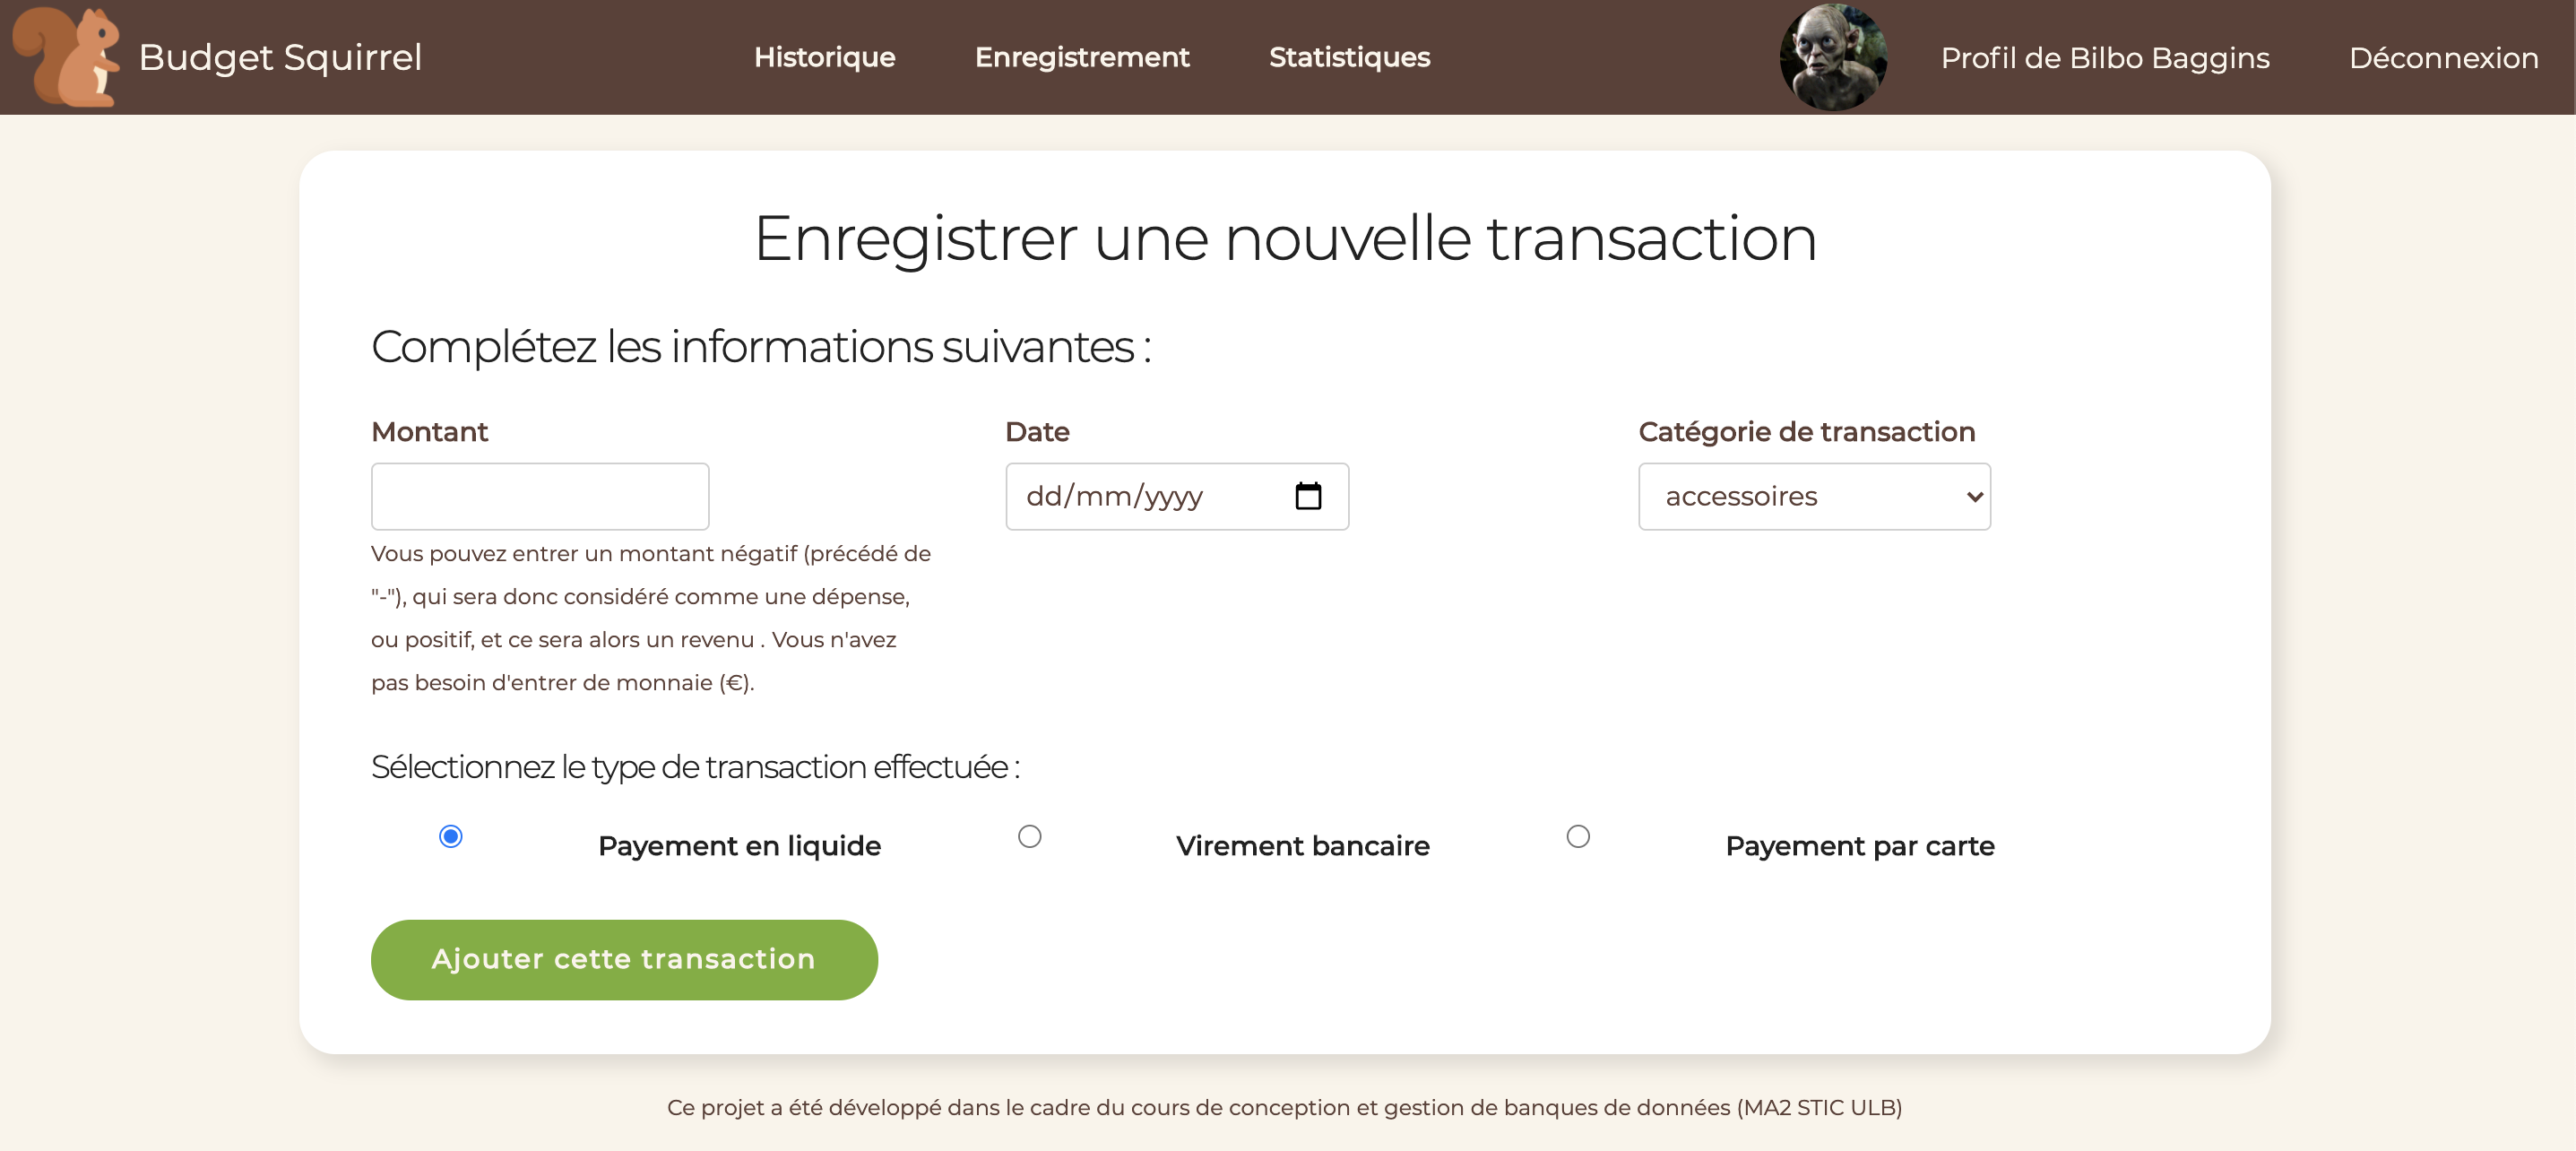
\includegraphics[scale=0.25]{enregistrement.png}}
\caption{\footnotesize{Enregistrement des transactions - Budget Squirrel}}
\end{figure}

La page historique, \verb\historique.php\, permet à l'utilisateur de visualiser les transactions effectuées : pour cela, il doit d'abord sélectionner le mois et l'année dont il veut consulter le budget.
Il a alors accès à un tableau affichant le montant, la date, la catégorie, et le type de transaction effectuée, et éventuellement la carte utilisée, le destinataire/bénéficiaire, et la communication.
En dessous de la table, l'utilisateur peut également voir le bilan total du mois. Enfin, il peut également choisir de supprimer une des transactions affichées.

\begin{figure}[!ht]
\noindent
\makebox[\textwidth][c]{
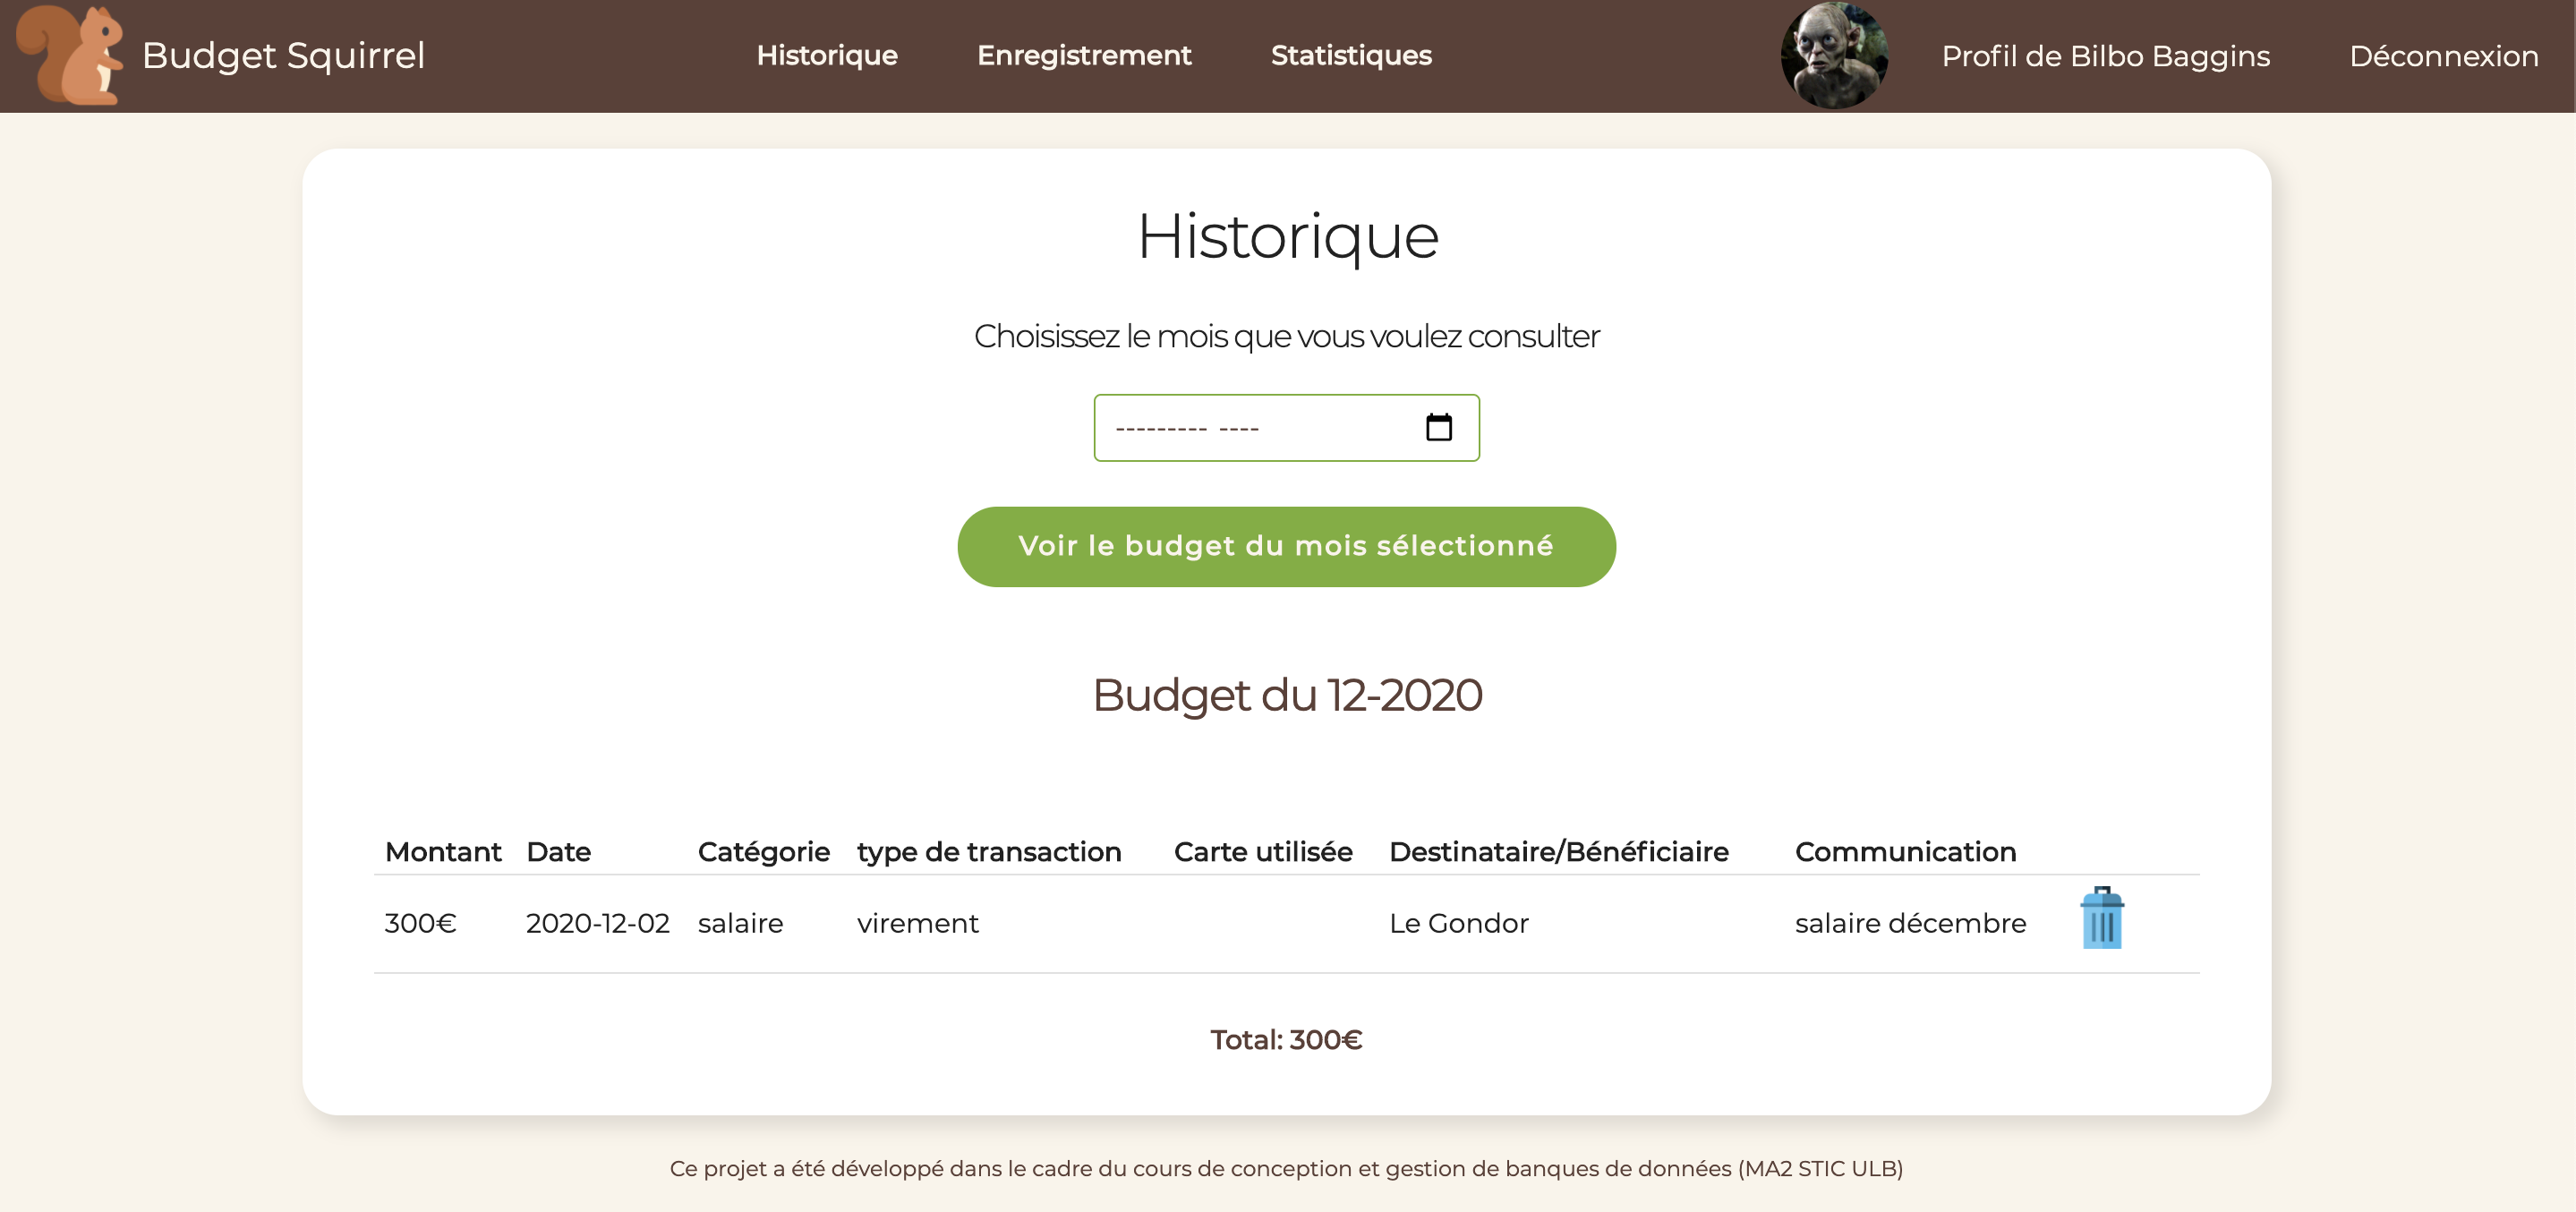
\includegraphics[scale=0.25]{historique.png}}
\caption{\footnotesize{Historique des transactions - Budget Squirrel}}
\end{figure}

L'écran de statistiques, \verb\stat.php\, offre différentes informations sur les données concernant l'utilisateur.
Les informations premières informations offertes sont les suivantes : un total des dépenses, un total des revenus, et un bilan.
Un tableau montrant la répartition des transactions (dépenses et revenus) par mois, ainsi que le bilan par mois, pour une vue plus condensée de l'historique, est également affiché, et accompagné de son graphique (généré en JavaScript) correspondant.
Un autre tableau montrant la répartition totale par catégorie, couplé à une description de chaque catégorie, est aussi accompagné de son graphique, cette fois-ci un diagramme circulaire. 
Enfin, la répartition des transactions entre les différents types de payements (le nombre d'utilisations, le bilan des dépenses et le bilan des revenus pour chaque type de transaction) est affiché.

\begin{figure}[!ht]
\noindent
\makebox[\textwidth][c]{
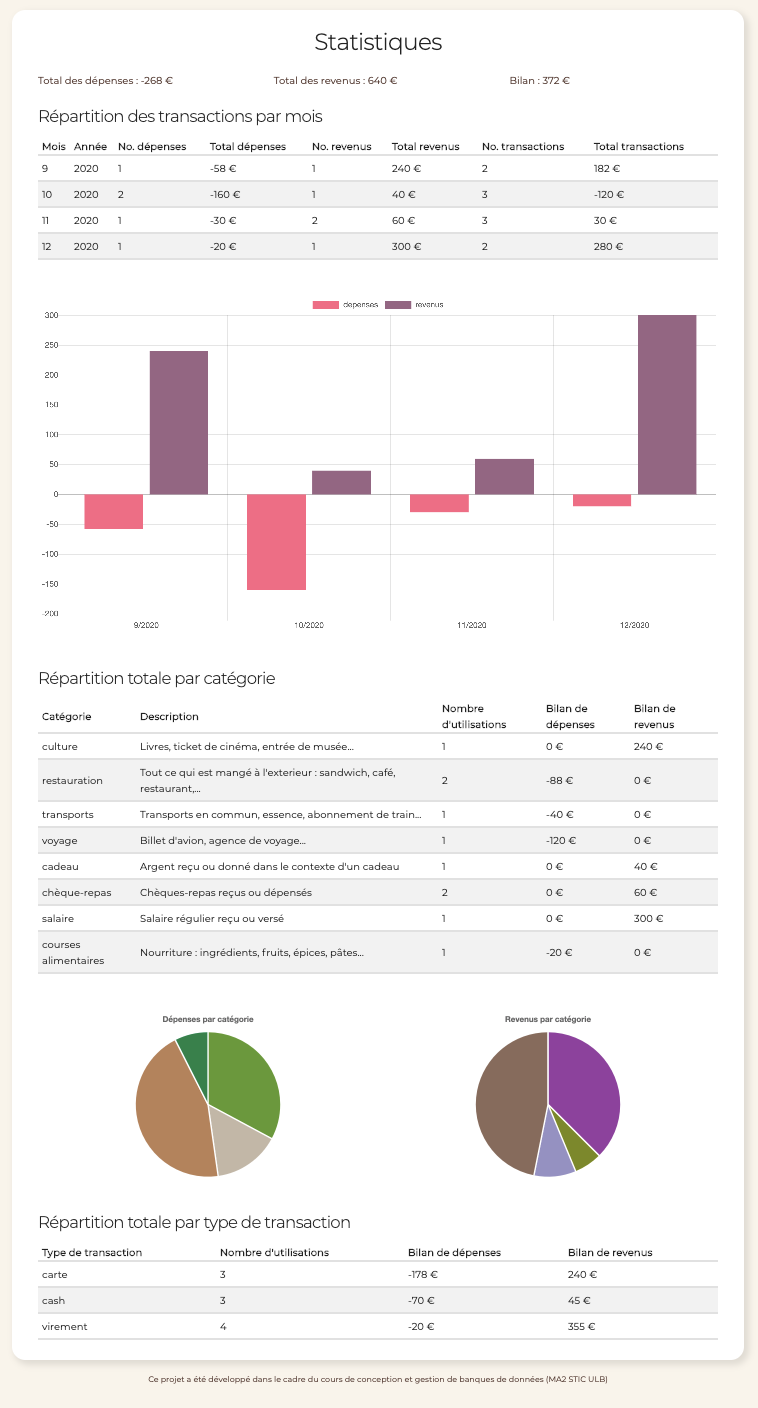
\includegraphics[scale=0.55]{stat.png}}
\caption{\footnotesize{Statistiques - Budget Squirrel}}
\end{figure}

À tout moment, l'utilisateur peut également se déconnecter, en cliquant, en haut à droite de la barre de navigation, sur \og déconnexion\fg .
Il est alors redirigé vers \verb\logout.php\.
Les informations de session (donc, le NISS sous lequel l'utilisateur est connecté) sont effacées, et l'utilisateur peut choisir de retourner à l'écran d'accueil pour se reconnecter ou s'inscrire.

\newpage

\section{Développement du projet}

Budget Squirrel est une application constituée d'une base des données et d'une interface client.
Le design, le développement et l'administration d'une telle application nécessitent donc une chorégraphie particulière, reposant sur des livrables qui doivent être prêts à l'emploi dans une certaine séquence, et qui se trouvent la plupart de temps dans une symbiose étroite.
De plus, certaines exigences du projet, établies ou agréées dès le départ, et révisées pendant les séances de guidance au projet, ainsi que certaines contraintes liées à d'autres engagements impératifs se sont vite imposées comme des conditions demandant une coordination ainsi qu'une communication ouverte et souple au sein du groupe.
Notre groupe s'est mis rapidement d'accord sur une division des tâches qui prend en compte les contraintes relatives aux disponibilités de chacune d'entre nous, ainsi qu'aux préférences des techniques et outils des développement, toute en gardant en vue l'impératif d'avoir touché au moins une fois à chaque écran et surtout d'avoir participé en tandem le plus que possible dans les parties couvrant la matière vue au cours.
Le développement de toutes les parties, de la conception de la base de donnée et des pages de l'application, en passant par le développement PHP, l'écriture de la base de donnée et des scripts SQL, jusqu'à l'écriture de ce rapport, s'est déroulé de manière organique, grâce à l'utilisation d'un repository github et d'un Google Drive commun, et de communications écrites et orales quasi-journalières permettant de faire le point sur notre avancement, nos difficultés, ainsi que l'état du projet.

\subsection{Travail conceptuel et outils employés pour démarrer le projet}

En suivant le calendrier communiqué au cours, nous avons fait une proposition de projet le 3 octobre, et avons reçu une confirmation pour le deuxième sujet dans un bref délai.

\begin{figure}[!ht]
\noindent
\makebox[\textwidth][c]{
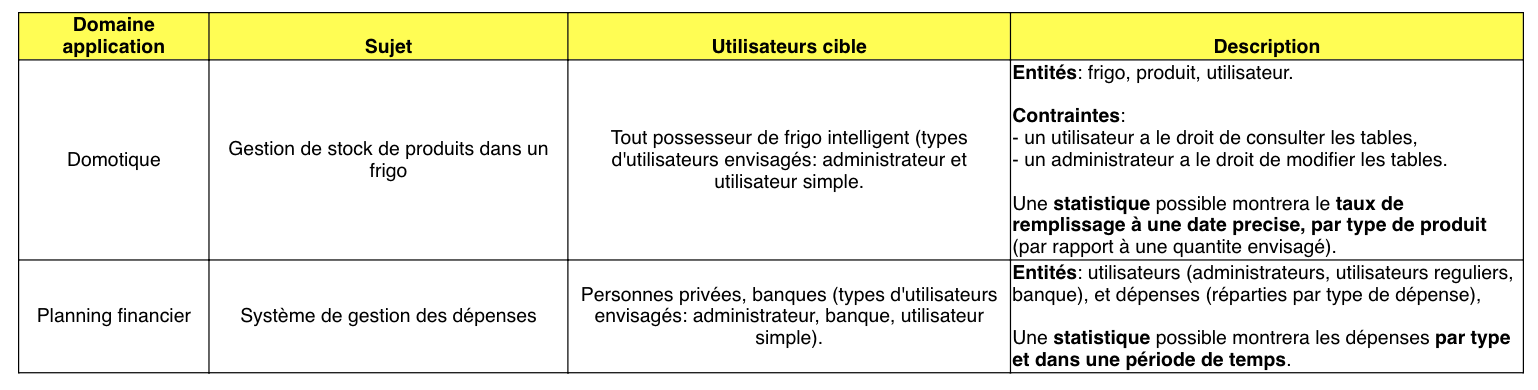
\includegraphics[scale=0.56]{proposal.png}}
\caption{\footnotesize{Sujets proposés en vue de développement}}
\end{figure}

Une fois le choix de projet validé, nous avons commencé le travail de conceptualisation, avec un double objectif: la conception d'un modèle entité-association, ainsi qu'une première ébauche d'interface client.
Pour nous aider dans la démarche EA, nous avons employé l'application web draw.io\footnote{\url{https://app.diagrams.net/}}.
En ce qui concerne l'interface client, l'outil Figma\footnote{\url{https://www.figma.com/}} à été employé dans la construction des maquettes.
Le résultat de ce travail s'est matérialisé dans un rapport préliminaire, présenté pour évaluation et validation le 31 octobre.
C'est en suivant ce rapport préliminaire que nous avons par la suite développé les éléments décrits dans les sections 2 et 3 du présent rapport.
 
\subsection{Design et techniques de travail }

La partie design à été facilitée par l'emploi d'une structure CSS ouverte\footnote{le boilerplate CSS Skeleton, \url{http://getskeleton.com/}}, que nous avons taillée aux besoins de notre application et combinée à une structure HTML.
Ensemble, les parties HTML et CSS du projet reprenaient (et amélioraient) notre premier design réalisé sur Figma, et posaient les bases de notre structure à compléter en y introduisant des éléments de PHP.
La section 5 du rapport témoigne des choix qui ont été gardés et implémentés au niveau du design de l'application.

L'étape de conception d'une application fonctionnelle a introduit une première couche de complexité en ce qui concerne l'imbrication des langages utilisés, en ajoutant PHP et HTML aux requêtes SQL.
Le PHP étant un langage très flexible, il nous a été relativement facile de créer de nombreuses contraintes côté client, et de combiner différentes requêtes SQL pour que l'application réponde exactement comme il faut à tout input de l'utilisateur, écrivant (et restreignant) les informations entrées du côté de l'application vers la base de données. 
Par contre, un des défis que nous avons rencontré durant le développement de ce projet a été l'écriture de données en utilisant du SQL pur, sans l'aide de l'application.
Certains éléments, facilement mis en place en PHP, étaient difficiles à traduire en SQL.
Ainsi, aux alentours de la moitié du développement, nous avons révisé notre script de création de base de données, afin que, comme l'application, il réponde exactement comme demandé par les contraintes établies dans les sections 2 et 3 : c'est ce qui a permis la création de la plupart de nos déclencheurs.
Finalement, l'application n'en est que plus solide, car les vérifications se font à deux niveaux lors de l'écriture de données via l'application : du côté client, et du côté de la base de données.

Une deuxième couche de complexité à été rajoutée par l'introduction des éléments JavaScript de visualisation dynamique des données (toggle screen, et graphes dynamiques) et des éléments en SQL d'agrégation des données (vues statistiques).
De manière générale, une des parties la plus difficile à été d'orchestrer, d'une façon robuste et cohérente, la partie d'insertions, mises à jour, et suppressions, afin d'éviter la perte des données, ou bien le double encodage.
Faire le choix entre l'ajout des contraintes au niveau de client, ou bien au niveau de la base des données, ainsi que naviguer entre les contraintes implémentées, n'a pas toujours été facile.
Pour parer ces difficultés nous avons employé la technique de programmation en binôme (asynchrone, en utilisant GitHub pour partager les mises à jours au niveau du code, et Teams pour faciliter la communication).
La taille restreinte du groupe à particulièrement facilité cette méthode de travail, et nous à permis une prise de décision rapide.

\newpage
\section{Conclusion}

Le principal défi de ce projet a finalement été d'assurer une cohérence entre la partie SQL et l'application PHP.
Le temps a également été un facteur qui a restreint notre développement, et nous avons parfois dû choisir d'aller au plus simple en ce qui concerne certains éléments du système développé.
Toutefois, grâce à ce projet, nous avons pu explorer concrètement différents aspects théoriques vus aux cours de base de données de master 1 et master 2, ce qui a été une expérience très enrichissante, et construire une application PHP relativement complète, couplée à une base de données possédant quelques éléments \og automatiques\fg (par exemple, la création automatisée de budgets mensuels). Nous pensons ainsi avoir acquis une meilleure compréhension de divers éléments de SQL, ainsi que développé des connaissances de base en PHP.

La présence de nombreuses ressources disponibles sur le web a été un avantage, mais aussi un inconvénient : pour les parties où nous avions le moins de connaissance, comme l'application concrète de déclencheurs, il nous a parfois été difficile de faire la part des choses à travers les nombreux conseils disponibles sur StackOverflow et d'autres ressources du même type.
La documentation officielle de PHP étant toutefois parfois assez obscure, StackOverflow a également été une ressource précieuse sans laquelle il nous aurait été plus difficile de développer certains éléments (de PHP, mais aussi de JavaScript).

Le système que nous rendons en l'état est bien sûr encore perfectible. Nous pensons notamment qu'il serait intéressant d'y apporter les améliorations suivantes, afin de le rendre plus robuste : 
\begin{itemize}
\item La vérification du NISS par rapport à la date de naissance de l'utilisateur, vu que les premiers chiffres du NISS correspondent à la date de naissance;
\item L'ajout d'une connexion par mot de passe pour l'utilisateur de l'application;
\item L'ajout d'une interface administrateur dans l'application;
\item La suppression du bilan dans la table budget mensuel : avec nos connaissances de départ, nous n'avions pas pu prévoir tout ce que permettaient les vues. Après le développement du système, nous nous rendons compte que finalement, \verb\budget_mensuel.bilan\ n'est pas réellement nécessaire;
\item Enfin, le choix de la matérialisation pour la traduction de l'héritage peut également être remis en question. Peut-être que conserver simplement la super-entité, ou encore seulement les sous-entités, aurait été plus adéquat dans notre système? Toutefois, ce choix nous a permis de comprendre concrètement l'impact des choix de traduction et de conceptualisation sur un système de base de données.
\end{itemize}

%voir si bibliographie nécessaire
%\chapter*{Bibliographie} 
%\addcontentsline{toc}{chapter}{Bibliographie}
%\markboth{Bibliographie}{}
%
%\printbibliography[heading=none]
%
%\fussy

%Voir si annexes nécessaire
%\chapter*{Annexes}
%\addcontentsline{toc}{chapter}{Annexes}
%\markboth{Annexes}{}

\end{document} % fin du corps du texte